\hypertarget{cmdInterpreter_8c}{
\section{cmd\-Interpreter.c File Reference}
\label{cmdInterpreter_8c}\index{cmdInterpreter.c@{cmdInterpreter.c}}
}
{\tt \#include $<$stdio.h$>$}\par
{\tt \#include $<$string.h$>$}\par
{\tt \#include \char`\"{}memoryguard.h\char`\"{}}\par
{\tt \#include $<$errno.h$>$}\par
{\tt \#include $<$sys/types.h$>$}\par
{\tt \#include $<$sys/stat.h$>$}\par
{\tt \#include $<$fcntl.h$>$}\par
{\tt \#include $<$unistd.h$>$}\par
{\tt \#include $<$time.h$>$}\par
{\tt \#include \char`\"{}cmd\-Interpreter.h\char`\"{}}\par
{\tt \#include \char`\"{}dcsc\-Msg\-Buffer\-Interface.h\char`\"{}}\par
{\tt \#include \char`\"{}selectmap\-Interface.h\char`\"{}}\par
{\tt \#include \char`\"{}mrtimers.h\char`\"{}}\par
{\tt \#include \char`\"{}mrshellprim.h\char`\"{}}\par


Include dependency graph for cmd\-Interpreter.c:\begin{figure}[H]
\begin{center}
\leavevmode
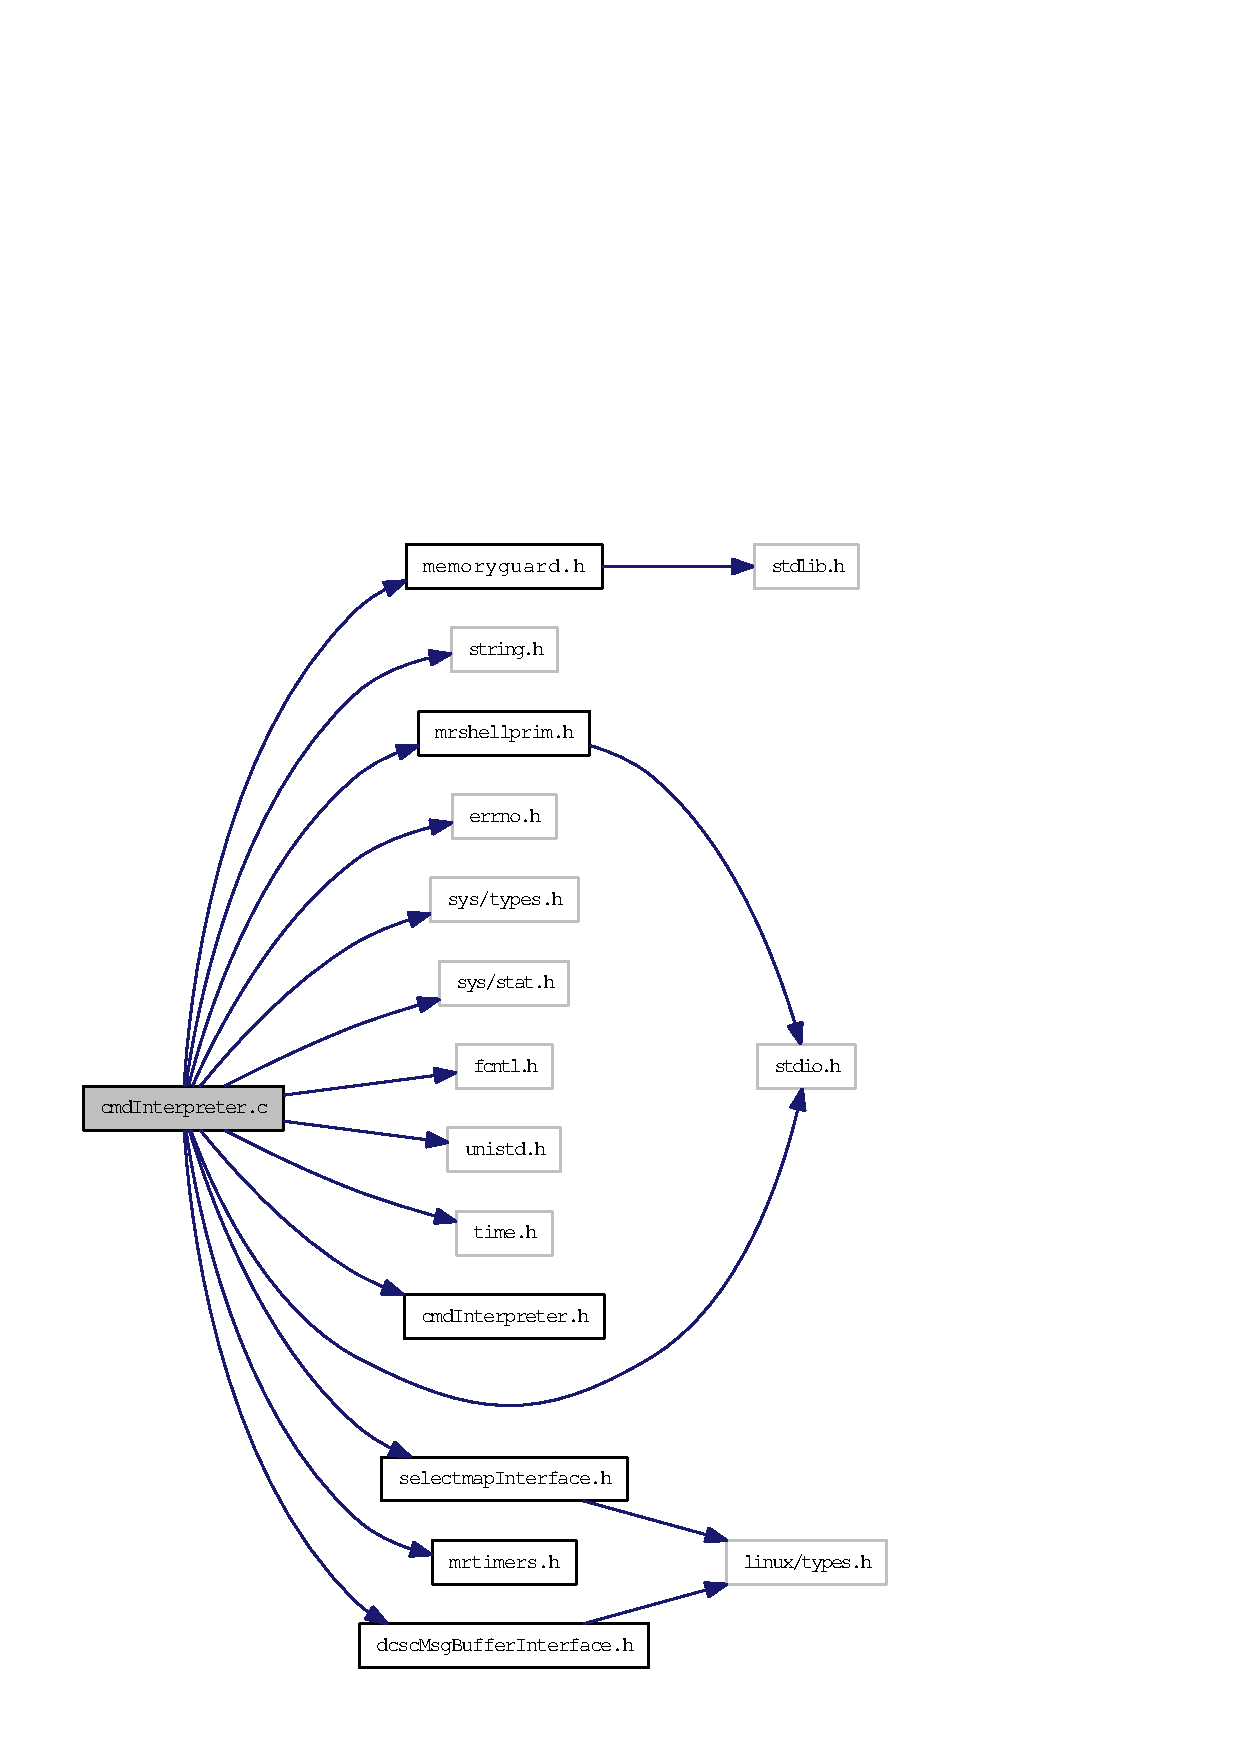
\includegraphics[width=215pt]{cmdInterpreter_8c__incl}
\end{center}
\end{figure}
\subsection*{Data Structures}
\begin{CompactItemize}
\item 
struct \hyperlink{structTCondition}{TCondition}
\end{CompactItemize}
\subsection*{Defines}
\begin{CompactItemize}
\item 
\#define \hyperlink{cmdInterpreter_8c_a2715fedb0c405a7e0062c79494b1ec0}{PRINT\_\-COMMAND\_\-BUFFER\_\-CTR\_\-STRING}~\char`\"{}pcb (print command buffer)\char`\"{}
\item 
\#define \hyperlink{cmdInterpreter_8c_982ee2112f9e2dccdaf82731415a0441}{PRINT\_\-RESULT\_\-BUFFER\_\-CTR\_\-STRING}~\char`\"{}prb (print result buffer)\char`\"{}
\item 
\#define \hyperlink{cmdInterpreter_8c_348a570c30753c168854ec146a2fb53d}{CHECK\_\-COMMAND\_\-BUFFER\_\-CTR\_\-STRING}~\char`\"{}c   (check command buffer)\char`\"{}
\item 
\#define \hyperlink{cmdInterpreter_8c_402f2e4e3254aa689123c78be75bed0a}{IGNORE\_\-BUFFER\_\-CHECK\_\-CTR\_\-STRING}~\char`\"{}i   (ignore buffer check)\char`\"{}
\item 
\#define \hyperlink{cmdInterpreter_8c_997f96a957fef1c6c614fb5cf4b4e3e2}{PRINT\_\-CTRL\_\-REGISTER\_\-CTR\_\-STRING}~\char`\"{}pcr (print control register)\char`\"{}
\item 
\#define \hyperlink{cmdInterpreter_8c_82cf9e89b90c524882e4c7ec0826a37f}{PRINT\_\-COMMAND\_\-RESULT\_\-CTR\_\-STRING}~\char`\"{}r   (print command result)\char`\"{}
\item 
\#define \hyperlink{cmdInterpreter_8c_c880e8e94aca75337b987af06141dcaa}{CMD\_\-STRING\_\-PROFILE}~\char`\"{}profile\char`\"{}
\item 
\#define \hyperlink{cmdInterpreter_8c_5d86dae553f9c8b404487c4f1d3592df}{CMD\_\-STRING\_\-MRT\_\-DEBUG}~\char`\"{}timerdbg\char`\"{}
\end{CompactItemize}
\subsection*{Enumerations}
\begin{CompactItemize}
\item 
enum \hyperlink{cmdInterpreter_8c_ab5835ceff4b64ce6db4148256e0a0f0}{Condition\-Types} \{ \hyperlink{cmdInterpreter_8c_ab5835ceff4b64ce6db4148256e0a0f067fd08219d48244557a06e13926853ee}{e\_\-fail} =  0, 
\hyperlink{cmdInterpreter_8c_ab5835ceff4b64ce6db4148256e0a0f0cb161923a23a717c2d959051d073d65c}{e\_\-continue}
 \}
\end{CompactItemize}
\subsection*{Functions}
\begin{CompactItemize}
\item 
void $\ast$ \hyperlink{cmdInterpreter_8c_46956baca790c8f97d618114d456b1fe}{Convert\-ASCII2Bin} (char $\ast$p\-ASCIIBuffer, int $\ast$pi\-Buffer\-Size, int i\-Word\-Size)
\item 
int \hyperlink{cmdInterpreter_8c_ac3ae2fb745e63e33060d5c0b658f745}{print\-Info} ()
\item 
void \hyperlink{cmdInterpreter_8c_15843554cb32ffb674f4245cfe5ee524}{print\-Debug\-Help} (int i\-Level)
\item 
int \hyperlink{cmdInterpreter_8c_f03f7609a66def2e7fae02a477c38d97}{print\-Help} ()
\item 
void \hyperlink{cmdInterpreter_8c_17ba9ebf0687897855a7c95f19e99c3d}{print\-Read\-Help} ()
\item 
void \hyperlink{cmdInterpreter_8c_c744cdcd05bdccf013ccbc82daa2282a}{print\-Batch\-Proc\-Help} ()
\item 
int \hyperlink{cmdInterpreter_8c_6ead18c93a106e1f1ba5871e908d9916}{read\-Time} (const char $\ast$$\ast$array\-Arg, int i\-Nof\-Args, int $\ast$p\-Sec, int $\ast$p\-Musec)
\item 
int \hyperlink{cmdInterpreter_8c_a78c9a935a342b0b7b9a3c9896c5e85b}{wait\-Condition} (const char $\ast$$\ast$array\-Arg, int i\-Nof\-Args)
\item 
int \hyperlink{cmdInterpreter_8c_f0155066c64e72c64ab000444db4fcad}{build\-Data\-Buffer\-From\-File} (const char $\ast$$\ast$array\-Arg, int nof\-Args, \_\-\_\-u32 $\ast$$\ast$pp\-Buffer, int $\ast$p\-Data\-Format, int i\-Mode)
\item 
int \hyperlink{cmdInterpreter_8c_6f67c6327e24c23440e0fdf83d06e41d}{exec\-Write\-Cmd} (const char $\ast$$\ast$array\-Arg, int i\-Nof\-Args, int i\-Mode)
\begin{CompactList}\small\item\em execute the write command there are 3 argument formats, the argument array is scanned and interpreted according to: 1. \item\end{CompactList}\item 
int \hyperlink{cmdInterpreter_8c_78a2282cf7d3dbf552e5f9876dba01cf}{Scan\-Coefficients} (const char $\ast$p\-Format, float $\ast$pf\-M, float $\ast$pf\-N, \_\-\_\-u32 $\ast$p\-Mask)
\item 
int \hyperlink{cmdInterpreter_8c_e3bcc6695f3c41940a8ab1f428101f07}{print\-Read\-Output\-Formatted} (unsigned char $\ast$\hyperlink{dcscMsgBufferInterface_8c_7fe69f55846ac3a138c130665f1f1e49}{p\-Buffer}, int i\-Buffer\-Size, const char $\ast$p\-Format, int i\-Start\-Address, FILE $\ast$fp)
\item 
int \hyperlink{cmdInterpreter_8c_a7c39db1bcd241c2ae5f259c0281abb6}{exec\-Read\-Cmd} (const char $\ast$$\ast$array\-Arg, int i\-Nof\-Args, int i\-Mode)
\item 
int \hyperlink{cmdInterpreter_8c_ac7fb947e83d5813fb30995133f29955}{timed\-Wait} (int i\-Wait\-Sec, int i\-Wait\-Musec)
\item 
int \hyperlink{cmdInterpreter_8c_ae37490e691f5b4d2c2e8f22713555da}{terminate\-Batch\-Processing} ()
\item 
int \hyperlink{cmdInterpreter_8c_0977826c2ae8c6c45ccfcfa1843cf83c}{exec\-Batch} (const char $\ast$$\ast$array\-Arg, int i\-Nof\-Args)
\item 
int \hyperlink{cmdInterpreter_8c_4a4e70ab937646237dbd0f0db81cdd99}{driver\-Ctrl\-Cmds} (\hyperlink{structArgDef__t}{TArg\-Def} $\ast$p\-Def, void $\ast$p\-User, FILE $\ast$p\-Out)
\item 
int \hyperlink{cmdInterpreter_8c_11ec76f8e60016409f2f33d10c70ef7e}{execute\-Main\-Commands} (const char $\ast$current\-Arg, const char $\ast$$\ast$array\-Arg, int i\-Nof\-Args, void $\ast$p\-User, FILE $\ast$p\-Out)
\item 
int \hyperlink{cmdInterpreter_8c_587fc3f8784e8339c998d9ca71bd7e12}{print\-Flash\-Help} ()
\item 
int \hyperlink{cmdInterpreter_8c_765eadf200d9f408461f7469c791d22c}{exec\-Flash\-Write\-Cmd} (const char $\ast$current\-Arg, const char $\ast$$\ast$array\-Arg, int i\-Nof\-Args, void $\ast$p\-User, FILE $\ast$p\-Out)
\item 
int \hyperlink{cmdInterpreter_8c_5df910c822508a5979806ec5d6548d65}{exec\-Flash\-Verify\-Cmd} (const char $\ast$current\-Arg, const char $\ast$$\ast$array\-Arg, int i\-Nof\-Args, void $\ast$p\-User, FILE $\ast$p\-Out)
\item 
int \hyperlink{cmdInterpreter_8c_0069fb7612546c23d35da357dd126984}{exec\-Flash\-Read\-Cmd} (const char $\ast$current\-Arg, const char $\ast$$\ast$array\-Arg, int i\-Nof\-Args, void $\ast$p\-User, FILE $\ast$p\-Out)
\item 
int \hyperlink{cmdInterpreter_8c_06be82b7d3ea06e8c4d3bc1aca1b63a1}{exec\-Flash\-Eraseall} ()
\item 
int \hyperlink{cmdInterpreter_8c_a4cd43e01e478de0f6dc0cec7ac6152b}{exec\-Flash\-Erase} (\hyperlink{structArgDef__t}{TArg\-Def} $\ast$p\-Def, void $\ast$p\-User, FILE $\ast$p\-Out)
\item 
int \hyperlink{cmdInterpreter_8c_a8f5aca148fba0272ac3acfee150f651}{exec\-Sm\-Write\-Reg} (const char $\ast$current\-Arg, const char $\ast$$\ast$array\-Arg, int i\-Nof\-Args, void $\ast$p\-User, FILE $\ast$p\-Out)
\item 
int \hyperlink{cmdInterpreter_8c_acf8d85528167524bef8a5e23b9ffd99}{exec\-Sm\-Read\-Reg} (const char $\ast$current\-Arg, const char $\ast$$\ast$array\-Arg, int i\-Nof\-Args, void $\ast$p\-User, FILE $\ast$p\-Out)
\item 
int \hyperlink{cmdInterpreter_8c_76b0a4b334ee64eb25b1637d709deb92}{print\-Selectmap\-Help} ()
\item 
int \hyperlink{cmdInterpreter_8c_69279ab735c2dc7e0a73d9c0bfe44f20}{print\-Firmware\-Help} ()
\item 
int \hyperlink{cmdInterpreter_8c_72ffcd5a8ec94bc388af9b6d9781f5de}{exec\-Reg\-Write\-Cmd} (const char $\ast$current\-Arg, const char $\ast$$\ast$array\-Arg, int i\-Nof\-Args, void $\ast$p\-User, FILE $\ast$p\-Out)
\item 
int \hyperlink{cmdInterpreter_8c_371d348f7b5d98c0ad4e7d6d20deb65c}{exec\-Reg\-Read\-Cmd} (const char $\ast$current\-Arg, const char $\ast$$\ast$array\-Arg, int i\-Nof\-Args, void $\ast$p\-User, FILE $\ast$p\-Out)
\item 
int \hyperlink{cmdInterpreter_8c_7c4a53b4c0e418e7102cba28b663fbb5}{ctrl\-Reg\-Status} ()
\item 
int \hyperlink{cmdInterpreter_8c_54cbd6e4f4a91310f0c408dc5c6b413d}{execute\-Command\-Args} (int i\-Nof\-Args, const char $\ast$$\ast$array\-Arg)
\item 
int \hyperlink{cmdInterpreter_8c_48086998882e7d163126de4100aa12ac}{execute\-Command\-Line} (char $\ast$p\-Cmd\-Line)
\end{CompactItemize}
\subsection*{Variables}
\begin{CompactItemize}
\item 
int \hyperlink{cmdInterpreter_8c_b1b44b602185677d4a2a372121627437}{g\_\-profiling} = 0
\item 
int \hyperlink{cmdInterpreter_8c_0aee2ec97f7e88992f9b2b333ca99be2}{g\_\-b\-Batch\-Processing} = 0
\item 
\hyperlink{structArgDef__t}{TArg\-Def} \hyperlink{cmdInterpreter_8c_083a182722ef62f10a68012ab6d7f707}{driver\-Ctrl\-Args} \mbox{[}$\,$\mbox{]}
\item 
\hyperlink{structFctArg__t}{TFct\-Arg} \hyperlink{cmdInterpreter_8c_3e75245c450c10d2323442d359f053d7}{driver\-Ctrl\-Desc}
\item 
\hyperlink{structFctMode__t}{TFct\-Mode} \hyperlink{cmdInterpreter_8c_fbc09bb85c6e4618a38dba855c588abd}{scan\-Mode\-Default} = \{SCANMODE\_\-FORCE\_\-TERMINATION, NULL, NULL\}
\item 
\hyperlink{structArgDef__t}{TArg\-Def} \hyperlink{cmdInterpreter_8c_4954a4ac4d6f82836d8b405a2ec86071}{selectmap\-Cmds} \mbox{[}$\,$\mbox{]}
\item 
\hyperlink{structArgDef__t}{TArg\-Def} \hyperlink{cmdInterpreter_8c_7399e2dab99f698c9275622762e94f74}{flash\-Erase\-Params} \mbox{[}$\,$\mbox{]}
\item 
\hyperlink{structFctArg__t}{TFct\-Arg} \hyperlink{cmdInterpreter_8c_9a757fd68a4d59000e0938fcdb423996}{flash\-Erase\-Desc}
\item 
\hyperlink{structArgDef__t}{TArg\-Def} \hyperlink{cmdInterpreter_8c_5a3ddbaacf0c338e408e3c0b55189d58}{flash\-Cmds} \mbox{[}$\,$\mbox{]}
\item 
\hyperlink{structArgDef__t}{TArg\-Def} \hyperlink{cmdInterpreter_8c_5a94aee581a390576806909f67968c30}{firmware\-Cmds} \mbox{[}$\,$\mbox{]}
\item 
\hyperlink{structArgDef__t}{TArg\-Def} \hyperlink{cmdInterpreter_8c_c1784239c15c2f1b5b4f1dbda9df65e7}{ctrl\-Reg\-Cmds} \mbox{[}$\,$\mbox{]}
\item 
\hyperlink{structArgDef__t}{TArg\-Def} \hyperlink{cmdInterpreter_8c_014d78494c13d4dc0430ee68de158559}{main\-Commands} \mbox{[}$\,$\mbox{]}
\end{CompactItemize}


\subsection{Define Documentation}
\hypertarget{cmdInterpreter_8c_348a570c30753c168854ec146a2fb53d}{
\index{cmdInterpreter.c@{cmd\-Interpreter.c}!CHECK_COMMAND_BUFFER_CTR_STRING@{CHECK\_\-COMMAND\_\-BUFFER\_\-CTR\_\-STRING}}
\index{CHECK_COMMAND_BUFFER_CTR_STRING@{CHECK\_\-COMMAND\_\-BUFFER\_\-CTR\_\-STRING}!cmdInterpreter.c@{cmd\-Interpreter.c}}
\subsubsection[CHECK\_\-COMMAND\_\-BUFFER\_\-CTR\_\-STRING]{\setlength{\rightskip}{0pt plus 5cm}\#define CHECK\_\-COMMAND\_\-BUFFER\_\-CTR\_\-STRING~\char`\"{}c   (check command buffer)\char`\"{}}}
\label{cmdInterpreter_8c_348a570c30753c168854ec146a2fb53d}




Definition at line 41 of file cmd\-Interpreter.c.\hypertarget{cmdInterpreter_8c_5d86dae553f9c8b404487c4f1d3592df}{
\index{cmdInterpreter.c@{cmd\-Interpreter.c}!CMD_STRING_MRT_DEBUG@{CMD\_\-STRING\_\-MRT\_\-DEBUG}}
\index{CMD_STRING_MRT_DEBUG@{CMD\_\-STRING\_\-MRT\_\-DEBUG}!cmdInterpreter.c@{cmd\-Interpreter.c}}
\subsubsection[CMD\_\-STRING\_\-MRT\_\-DEBUG]{\setlength{\rightskip}{0pt plus 5cm}\#define CMD\_\-STRING\_\-MRT\_\-DEBUG~\char`\"{}timerdbg\char`\"{}}}
\label{cmdInterpreter_8c_5d86dae553f9c8b404487c4f1d3592df}




Definition at line 46 of file cmd\-Interpreter.c.

Referenced by execute\-Main\-Commands().\hypertarget{cmdInterpreter_8c_c880e8e94aca75337b987af06141dcaa}{
\index{cmdInterpreter.c@{cmd\-Interpreter.c}!CMD_STRING_PROFILE@{CMD\_\-STRING\_\-PROFILE}}
\index{CMD_STRING_PROFILE@{CMD\_\-STRING\_\-PROFILE}!cmdInterpreter.c@{cmd\-Interpreter.c}}
\subsubsection[CMD\_\-STRING\_\-PROFILE]{\setlength{\rightskip}{0pt plus 5cm}\#define CMD\_\-STRING\_\-PROFILE~\char`\"{}profile\char`\"{}}}
\label{cmdInterpreter_8c_c880e8e94aca75337b987af06141dcaa}




Definition at line 45 of file cmd\-Interpreter.c.

Referenced by execute\-Main\-Commands().\hypertarget{cmdInterpreter_8c_402f2e4e3254aa689123c78be75bed0a}{
\index{cmdInterpreter.c@{cmd\-Interpreter.c}!IGNORE_BUFFER_CHECK_CTR_STRING@{IGNORE\_\-BUFFER\_\-CHECK\_\-CTR\_\-STRING}}
\index{IGNORE_BUFFER_CHECK_CTR_STRING@{IGNORE\_\-BUFFER\_\-CHECK\_\-CTR\_\-STRING}!cmdInterpreter.c@{cmd\-Interpreter.c}}
\subsubsection[IGNORE\_\-BUFFER\_\-CHECK\_\-CTR\_\-STRING]{\setlength{\rightskip}{0pt plus 5cm}\#define IGNORE\_\-BUFFER\_\-CHECK\_\-CTR\_\-STRING~\char`\"{}i   (ignore buffer check)\char`\"{}}}
\label{cmdInterpreter_8c_402f2e4e3254aa689123c78be75bed0a}




Definition at line 42 of file cmd\-Interpreter.c.\hypertarget{cmdInterpreter_8c_a2715fedb0c405a7e0062c79494b1ec0}{
\index{cmdInterpreter.c@{cmd\-Interpreter.c}!PRINT_COMMAND_BUFFER_CTR_STRING@{PRINT\_\-COMMAND\_\-BUFFER\_\-CTR\_\-STRING}}
\index{PRINT_COMMAND_BUFFER_CTR_STRING@{PRINT\_\-COMMAND\_\-BUFFER\_\-CTR\_\-STRING}!cmdInterpreter.c@{cmd\-Interpreter.c}}
\subsubsection[PRINT\_\-COMMAND\_\-BUFFER\_\-CTR\_\-STRING]{\setlength{\rightskip}{0pt plus 5cm}\#define PRINT\_\-COMMAND\_\-BUFFER\_\-CTR\_\-STRING~\char`\"{}pcb (print command buffer)\char`\"{}}}
\label{cmdInterpreter_8c_a2715fedb0c405a7e0062c79494b1ec0}




Definition at line 39 of file cmd\-Interpreter.c.\hypertarget{cmdInterpreter_8c_82cf9e89b90c524882e4c7ec0826a37f}{
\index{cmdInterpreter.c@{cmd\-Interpreter.c}!PRINT_COMMAND_RESULT_CTR_STRING@{PRINT\_\-COMMAND\_\-RESULT\_\-CTR\_\-STRING}}
\index{PRINT_COMMAND_RESULT_CTR_STRING@{PRINT\_\-COMMAND\_\-RESULT\_\-CTR\_\-STRING}!cmdInterpreter.c@{cmd\-Interpreter.c}}
\subsubsection[PRINT\_\-COMMAND\_\-RESULT\_\-CTR\_\-STRING]{\setlength{\rightskip}{0pt plus 5cm}\#define PRINT\_\-COMMAND\_\-RESULT\_\-CTR\_\-STRING~\char`\"{}r   (print command result)\char`\"{}}}
\label{cmdInterpreter_8c_82cf9e89b90c524882e4c7ec0826a37f}




Definition at line 44 of file cmd\-Interpreter.c.\hypertarget{cmdInterpreter_8c_997f96a957fef1c6c614fb5cf4b4e3e2}{
\index{cmdInterpreter.c@{cmd\-Interpreter.c}!PRINT_CTRL_REGISTER_CTR_STRING@{PRINT\_\-CTRL\_\-REGISTER\_\-CTR\_\-STRING}}
\index{PRINT_CTRL_REGISTER_CTR_STRING@{PRINT\_\-CTRL\_\-REGISTER\_\-CTR\_\-STRING}!cmdInterpreter.c@{cmd\-Interpreter.c}}
\subsubsection[PRINT\_\-CTRL\_\-REGISTER\_\-CTR\_\-STRING]{\setlength{\rightskip}{0pt plus 5cm}\#define PRINT\_\-CTRL\_\-REGISTER\_\-CTR\_\-STRING~\char`\"{}pcr (print control register)\char`\"{}}}
\label{cmdInterpreter_8c_997f96a957fef1c6c614fb5cf4b4e3e2}




Definition at line 43 of file cmd\-Interpreter.c.\hypertarget{cmdInterpreter_8c_982ee2112f9e2dccdaf82731415a0441}{
\index{cmdInterpreter.c@{cmd\-Interpreter.c}!PRINT_RESULT_BUFFER_CTR_STRING@{PRINT\_\-RESULT\_\-BUFFER\_\-CTR\_\-STRING}}
\index{PRINT_RESULT_BUFFER_CTR_STRING@{PRINT\_\-RESULT\_\-BUFFER\_\-CTR\_\-STRING}!cmdInterpreter.c@{cmd\-Interpreter.c}}
\subsubsection[PRINT\_\-RESULT\_\-BUFFER\_\-CTR\_\-STRING]{\setlength{\rightskip}{0pt plus 5cm}\#define PRINT\_\-RESULT\_\-BUFFER\_\-CTR\_\-STRING~\char`\"{}prb (print result buffer)\char`\"{}}}
\label{cmdInterpreter_8c_982ee2112f9e2dccdaf82731415a0441}




Definition at line 40 of file cmd\-Interpreter.c.

\subsection{Enumeration Type Documentation}
\hypertarget{cmdInterpreter_8c_ab5835ceff4b64ce6db4148256e0a0f0}{
\index{cmdInterpreter.c@{cmd\-Interpreter.c}!ConditionTypes@{ConditionTypes}}
\index{ConditionTypes@{ConditionTypes}!cmdInterpreter.c@{cmd\-Interpreter.c}}
\subsubsection[ConditionTypes]{\setlength{\rightskip}{0pt plus 5cm}enum \hyperlink{cmdInterpreter_8c_ab5835ceff4b64ce6db4148256e0a0f0}{Condition\-Types}}}
\label{cmdInterpreter_8c_ab5835ceff4b64ce6db4148256e0a0f0}


\begin{Desc}
\item[Enumerator: ]\par
\begin{description}
\index{e_fail@{e\_\-fail}!cmdInterpreter.c@{cmdInterpreter.c}}\index{cmdInterpreter.c@{cmdInterpreter.c}!e_fail@{e\_\-fail}}\item[{\em 
\hypertarget{cmdInterpreter_8c_ab5835ceff4b64ce6db4148256e0a0f067fd08219d48244557a06e13926853ee}{
e\_\-fail}
\label{cmdInterpreter_8c_ab5835ceff4b64ce6db4148256e0a0f067fd08219d48244557a06e13926853ee}
}]\index{e_continue@{e\_\-continue}!cmdInterpreter.c@{cmdInterpreter.c}}\index{cmdInterpreter.c@{cmdInterpreter.c}!e_continue@{e\_\-continue}}\item[{\em 
\hypertarget{cmdInterpreter_8c_ab5835ceff4b64ce6db4148256e0a0f0cb161923a23a717c2d959051d073d65c}{
e\_\-continue}
\label{cmdInterpreter_8c_ab5835ceff4b64ce6db4148256e0a0f0cb161923a23a717c2d959051d073d65c}
}]\end{description}
\end{Desc}



Definition at line 73 of file cmd\-Interpreter.c.

\subsection{Function Documentation}
\hypertarget{cmdInterpreter_8c_f0155066c64e72c64ab000444db4fcad}{
\index{cmdInterpreter.c@{cmd\-Interpreter.c}!buildDataBufferFromFile@{buildDataBufferFromFile}}
\index{buildDataBufferFromFile@{buildDataBufferFromFile}!cmdInterpreter.c@{cmd\-Interpreter.c}}
\subsubsection[buildDataBufferFromFile]{\setlength{\rightskip}{0pt plus 5cm}int build\-Data\-Buffer\-From\-File (const char $\ast$$\ast$ {\em array\-Arg}, int {\em nof\-Args}, \_\-\_\-u32 $\ast$$\ast$ {\em pp\-Buffer}, int $\ast$ {\em p\-Data\-Format}, int {\em i\-Mode})}}
\label{cmdInterpreter_8c_f0155066c64e72c64ab000444db4fcad}




Definition at line 490 of file cmd\-Interpreter.c.

References Convert\-ASCII2Bin(), DBG\_\-FILE\_\-CONVERT, get\-Dec\-Number\-From\-Arg(), and set\-Debug\-Option\-Flag().

Referenced by exec\-Write\-Cmd().

Here is the call graph for this function:\begin{figure}[H]
\begin{center}
\leavevmode
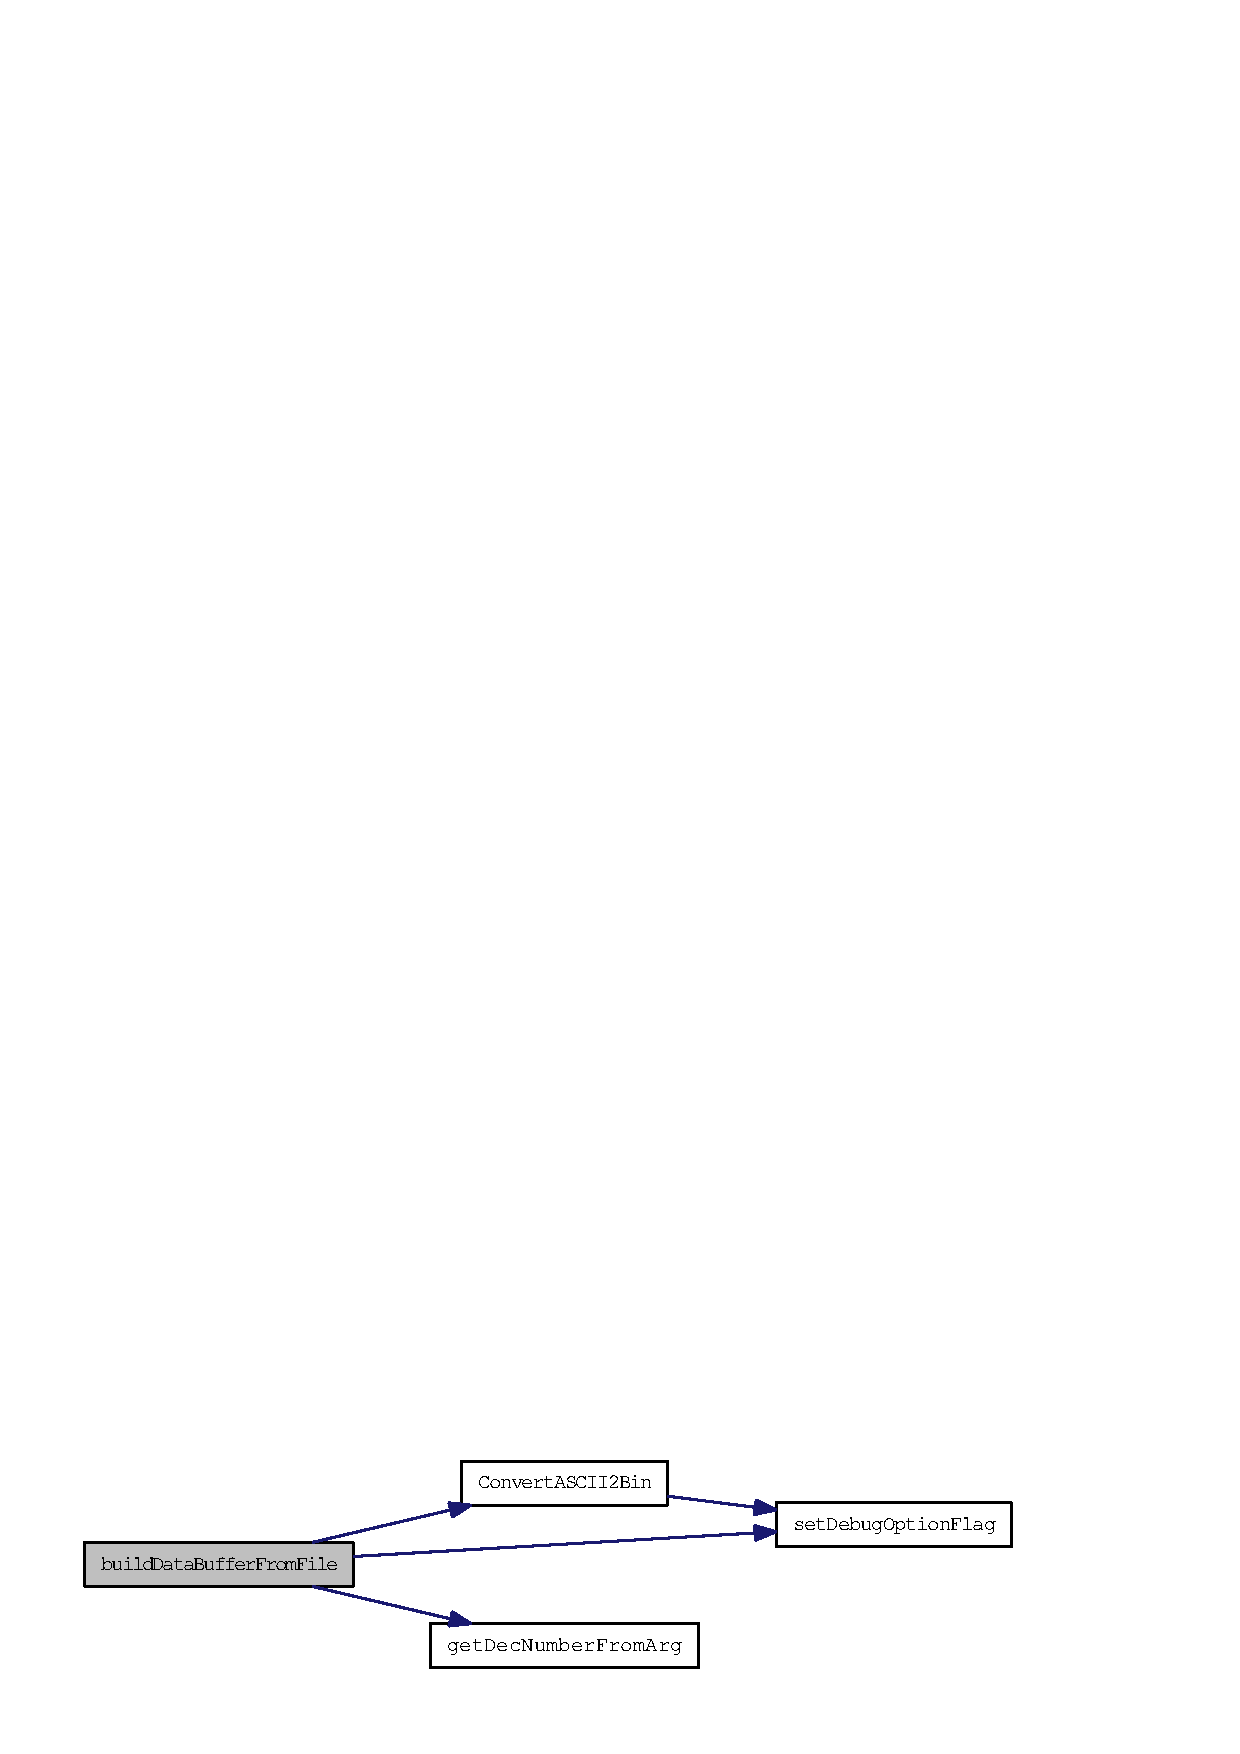
\includegraphics[width=245pt]{cmdInterpreter_8c_f0155066c64e72c64ab000444db4fcad_cgraph}
\end{center}
\end{figure}
\hypertarget{cmdInterpreter_8c_46956baca790c8f97d618114d456b1fe}{
\index{cmdInterpreter.c@{cmd\-Interpreter.c}!ConvertASCII2Bin@{ConvertASCII2Bin}}
\index{ConvertASCII2Bin@{ConvertASCII2Bin}!cmdInterpreter.c@{cmd\-Interpreter.c}}
\subsubsection[ConvertASCII2Bin]{\setlength{\rightskip}{0pt plus 5cm}void$\ast$ Convert\-ASCII2Bin (char $\ast$ {\em p\-ASCIIBuffer}, int $\ast$ {\em pi\-Buffer\-Size}, int {\em i\-Word\-Size})}}
\label{cmdInterpreter_8c_46956baca790c8f97d618114d456b1fe}




Definition at line 84 of file cmd\-Interpreter.c.

References DBG\_\-FILE\_\-CONVERT, and set\-Debug\-Option\-Flag().

Referenced by build\-Data\-Buffer\-From\-File().

Here is the call graph for this function:\begin{figure}[H]
\begin{center}
\leavevmode
\includegraphics[width=147pt]{cmdInterpreter_8c_46956baca790c8f97d618114d456b1fe_cgraph}
\end{center}
\end{figure}
\hypertarget{cmdInterpreter_8c_7c4a53b4c0e418e7102cba28b663fbb5}{
\index{cmdInterpreter.c@{cmd\-Interpreter.c}!ctrlRegStatus@{ctrlRegStatus}}
\index{ctrlRegStatus@{ctrlRegStatus}!cmdInterpreter.c@{cmd\-Interpreter.c}}
\subsubsection[ctrlRegStatus]{\setlength{\rightskip}{0pt plus 5cm}int ctrl\-Reg\-Status ()}}
\label{cmdInterpreter_8c_7c4a53b4c0e418e7102cba28b663fbb5}




Definition at line 1816 of file cmd\-Interpreter.c.

References e\-Read\-Ctrl\-Reg, and rcu\-Bus\-Control\-Cmd().

Here is the call graph for this function:\begin{figure}[H]
\begin{center}
\leavevmode
\includegraphics[width=212pt]{cmdInterpreter_8c_7c4a53b4c0e418e7102cba28b663fbb5_cgraph}
\end{center}
\end{figure}
\hypertarget{cmdInterpreter_8c_4a4e70ab937646237dbd0f0db81cdd99}{
\index{cmdInterpreter.c@{cmd\-Interpreter.c}!driverCtrlCmds@{driverCtrlCmds}}
\index{driverCtrlCmds@{driverCtrlCmds}!cmdInterpreter.c@{cmd\-Interpreter.c}}
\subsubsection[driverCtrlCmds]{\setlength{\rightskip}{0pt plus 5cm}int driver\-Ctrl\-Cmds (\hyperlink{structArgDef__t}{TArg\-Def} $\ast$ {\em p\-Def}, void $\ast$ {\em p\-User}, FILE $\ast$ {\em p\-Out})}}
\label{cmdInterpreter_8c_4a4e70ab937646237dbd0f0db81cdd99}




Definition at line 1445 of file cmd\-Interpreter.c.

References ARGPROC\_\-EXISTS, dcsc\-Driver\-Debug(), and mr\-Shell\-Prim\-Get\-Hex().

Here is the call graph for this function:\begin{figure}[H]
\begin{center}
\leavevmode
\includegraphics[width=215pt]{cmdInterpreter_8c_4a4e70ab937646237dbd0f0db81cdd99_cgraph}
\end{center}
\end{figure}
\hypertarget{cmdInterpreter_8c_0977826c2ae8c6c45ccfcfa1843cf83c}{
\index{cmdInterpreter.c@{cmd\-Interpreter.c}!execBatch@{execBatch}}
\index{execBatch@{execBatch}!cmdInterpreter.c@{cmd\-Interpreter.c}}
\subsubsection[execBatch]{\setlength{\rightskip}{0pt plus 5cm}int exec\-Batch (const char $\ast$$\ast$ {\em array\-Arg}, int {\em i\-Nof\-Args})}}
\label{cmdInterpreter_8c_0977826c2ae8c6c45ccfcfa1843cf83c}




Definition at line 1294 of file cmd\-Interpreter.c.

References execute\-Command\-Line(), g\_\-b\-Batch\-Processing, g\_\-profiling, get\-Dec\-Number\-From\-Arg(), get\-Timer\-Value\-String(), read\-Time(), remove\-Prec\-And\-Trailing\-Spec\-Chars(), start\-Timer(), stop\-Timer(), and timed\-Wait().

Referenced by execute\-Main\-Commands().

Here is the call graph for this function:\begin{figure}[H]
\begin{center}
\leavevmode
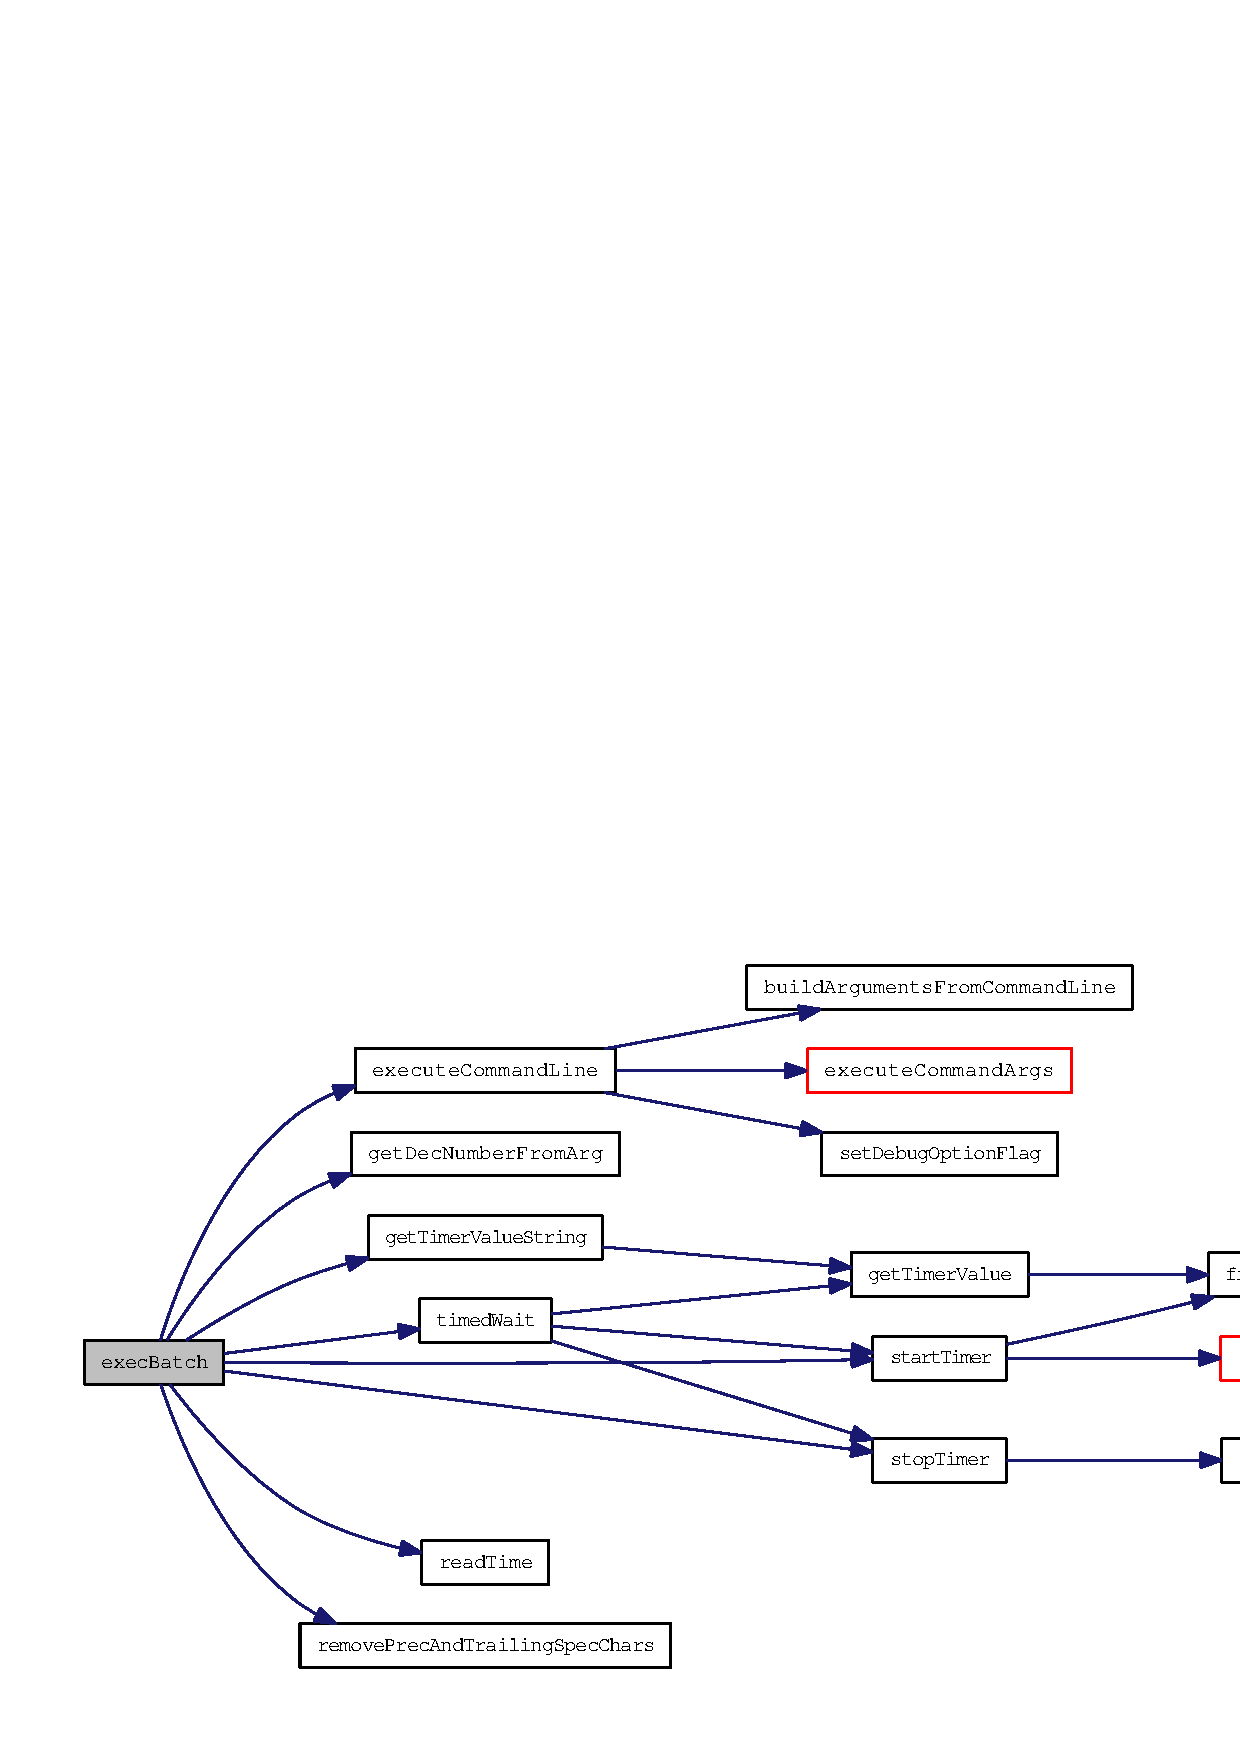
\includegraphics[width=335pt]{cmdInterpreter_8c_0977826c2ae8c6c45ccfcfa1843cf83c_cgraph}
\end{center}
\end{figure}
\hypertarget{cmdInterpreter_8c_a4cd43e01e478de0f6dc0cec7ac6152b}{
\index{cmdInterpreter.c@{cmd\-Interpreter.c}!execFlashErase@{execFlashErase}}
\index{execFlashErase@{execFlashErase}!cmdInterpreter.c@{cmd\-Interpreter.c}}
\subsubsection[execFlashErase]{\setlength{\rightskip}{0pt plus 5cm}int exec\-Flash\-Erase (\hyperlink{structArgDef__t}{TArg\-Def} $\ast$ {\em p\-Def}, void $\ast$ {\em p\-User}, FILE $\ast$ {\em p\-Out})}}
\label{cmdInterpreter_8c_a4cd43e01e478de0f6dc0cec7ac6152b}




Definition at line 1723 of file cmd\-Interpreter.c.

References ARGPROC\_\-EXISTS, mr\-Shell\-Prim\-Get\-Hex(), mr\-Shell\-Prim\-Get\-Int(), and rcu\-Flash\-Erase().

Here is the call graph for this function:\begin{figure}[H]
\begin{center}
\leavevmode
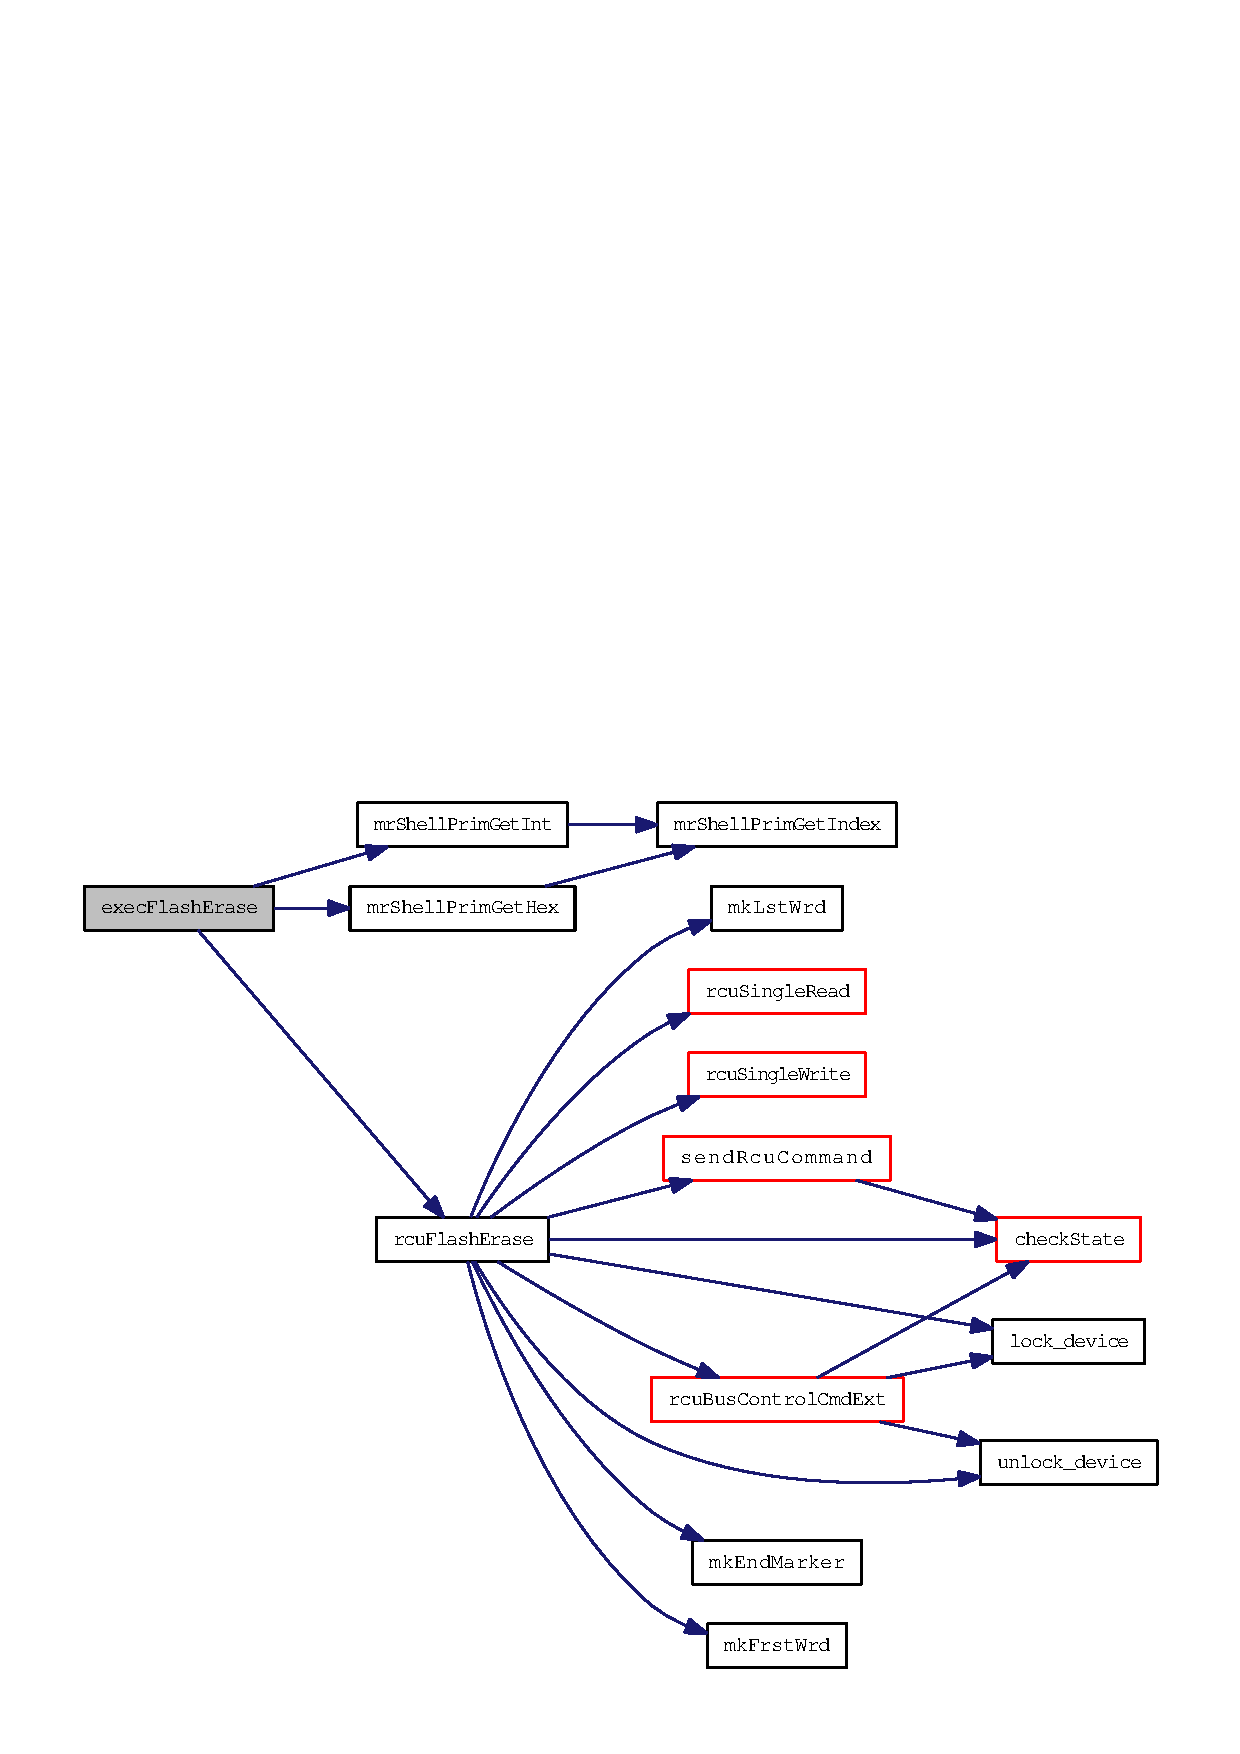
\includegraphics[width=280pt]{cmdInterpreter_8c_a4cd43e01e478de0f6dc0cec7ac6152b_cgraph}
\end{center}
\end{figure}
\hypertarget{cmdInterpreter_8c_06be82b7d3ea06e8c4d3bc1aca1b63a1}{
\index{cmdInterpreter.c@{cmd\-Interpreter.c}!execFlashEraseall@{execFlashEraseall}}
\index{execFlashEraseall@{execFlashEraseall}!cmdInterpreter.c@{cmd\-Interpreter.c}}
\subsubsection[execFlashEraseall]{\setlength{\rightskip}{0pt plus 5cm}int exec\-Flash\-Eraseall ()}}
\label{cmdInterpreter_8c_06be82b7d3ea06e8c4d3bc1aca1b63a1}




Definition at line 1718 of file cmd\-Interpreter.c.

References rcu\-Flash\-Erase().

Here is the call graph for this function:\begin{figure}[H]
\begin{center}
\leavevmode
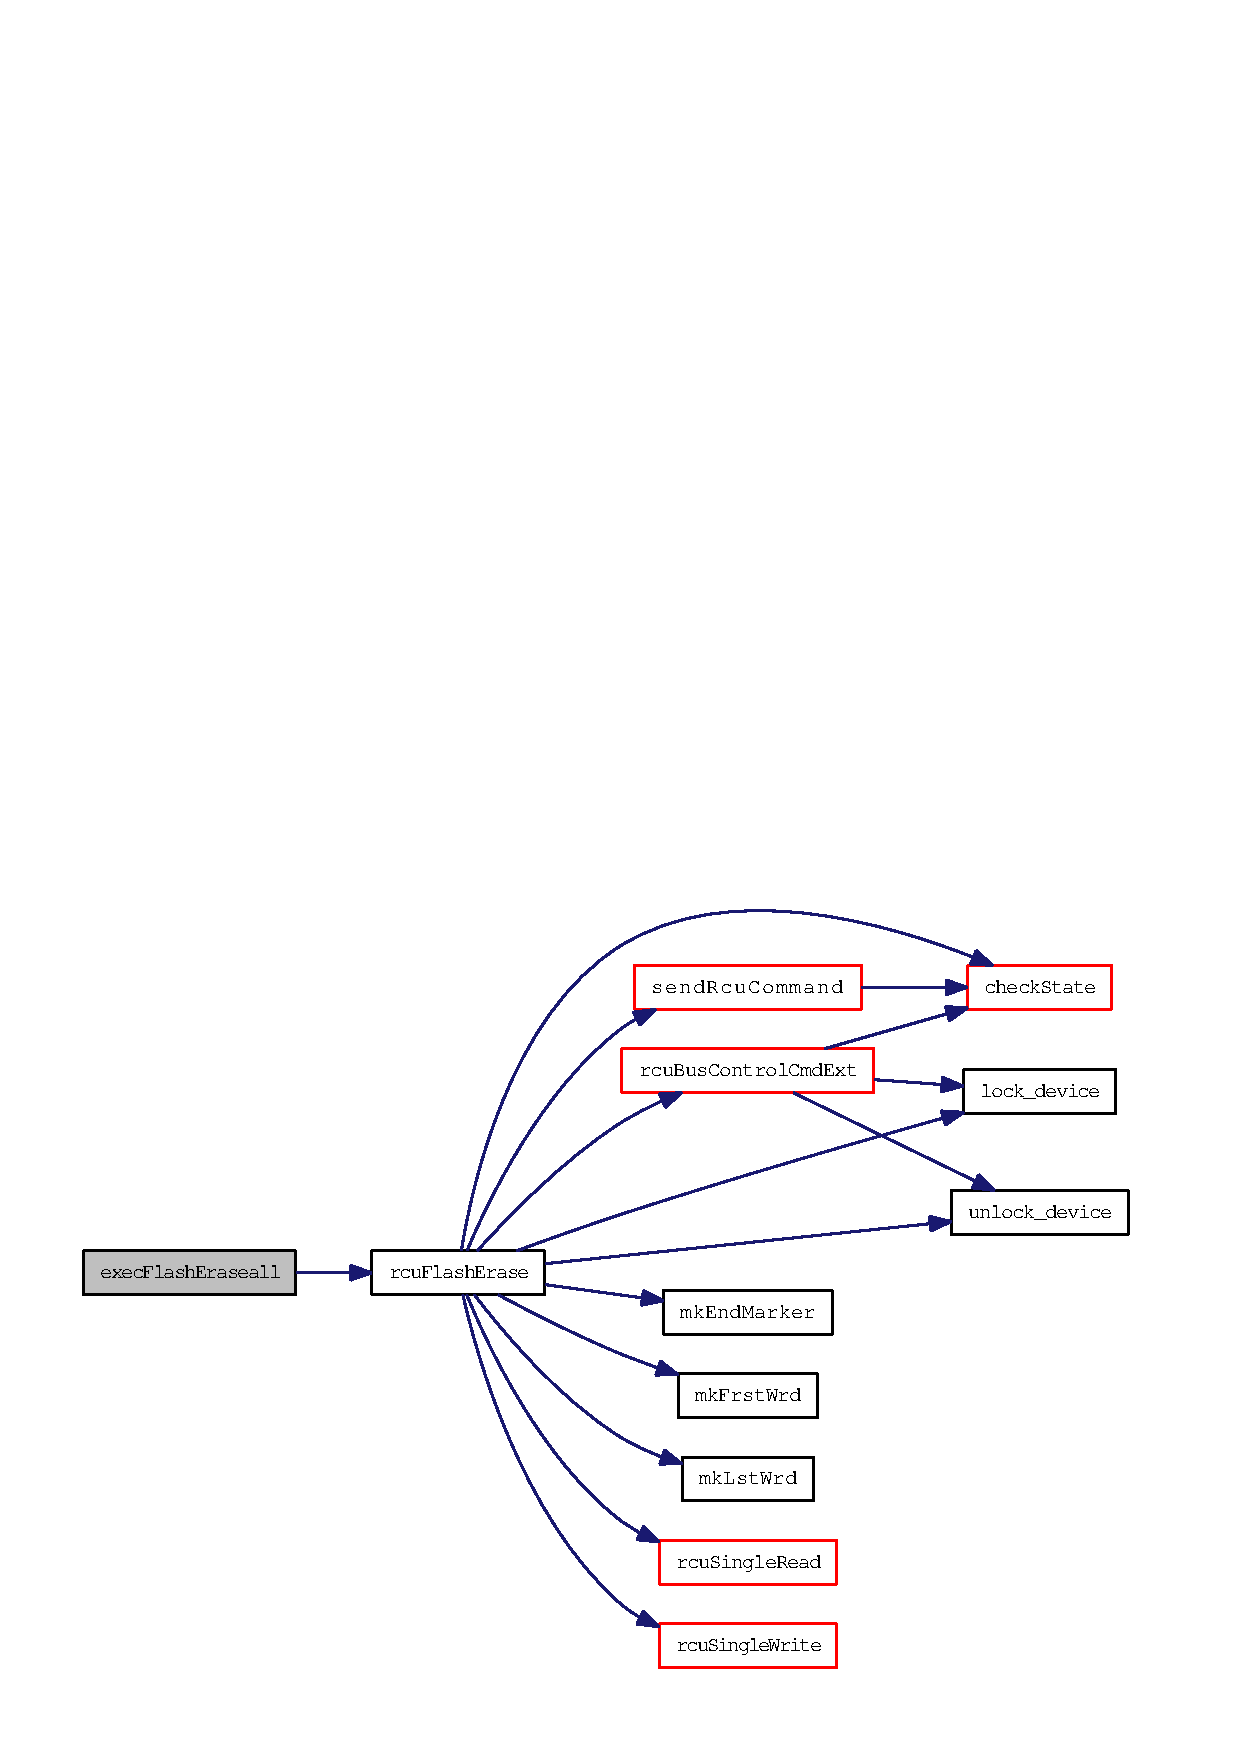
\includegraphics[width=273pt]{cmdInterpreter_8c_06be82b7d3ea06e8c4d3bc1aca1b63a1_cgraph}
\end{center}
\end{figure}
\hypertarget{cmdInterpreter_8c_0069fb7612546c23d35da357dd126984}{
\index{cmdInterpreter.c@{cmd\-Interpreter.c}!execFlashReadCmd@{execFlashReadCmd}}
\index{execFlashReadCmd@{execFlashReadCmd}!cmdInterpreter.c@{cmd\-Interpreter.c}}
\subsubsection[execFlashReadCmd]{\setlength{\rightskip}{0pt plus 5cm}int exec\-Flash\-Read\-Cmd (const char $\ast$ {\em current\-Arg}, const char $\ast$$\ast$ {\em array\-Arg}, int {\em i\-Nof\-Args}, void $\ast$ {\em p\-User}, FILE $\ast$ {\em p\-Out})}}
\label{cmdInterpreter_8c_0069fb7612546c23d35da357dd126984}




Definition at line 1711 of file cmd\-Interpreter.c.

References exec\-Read\-Cmd().

Here is the call graph for this function:\begin{figure}[H]
\begin{center}
\leavevmode
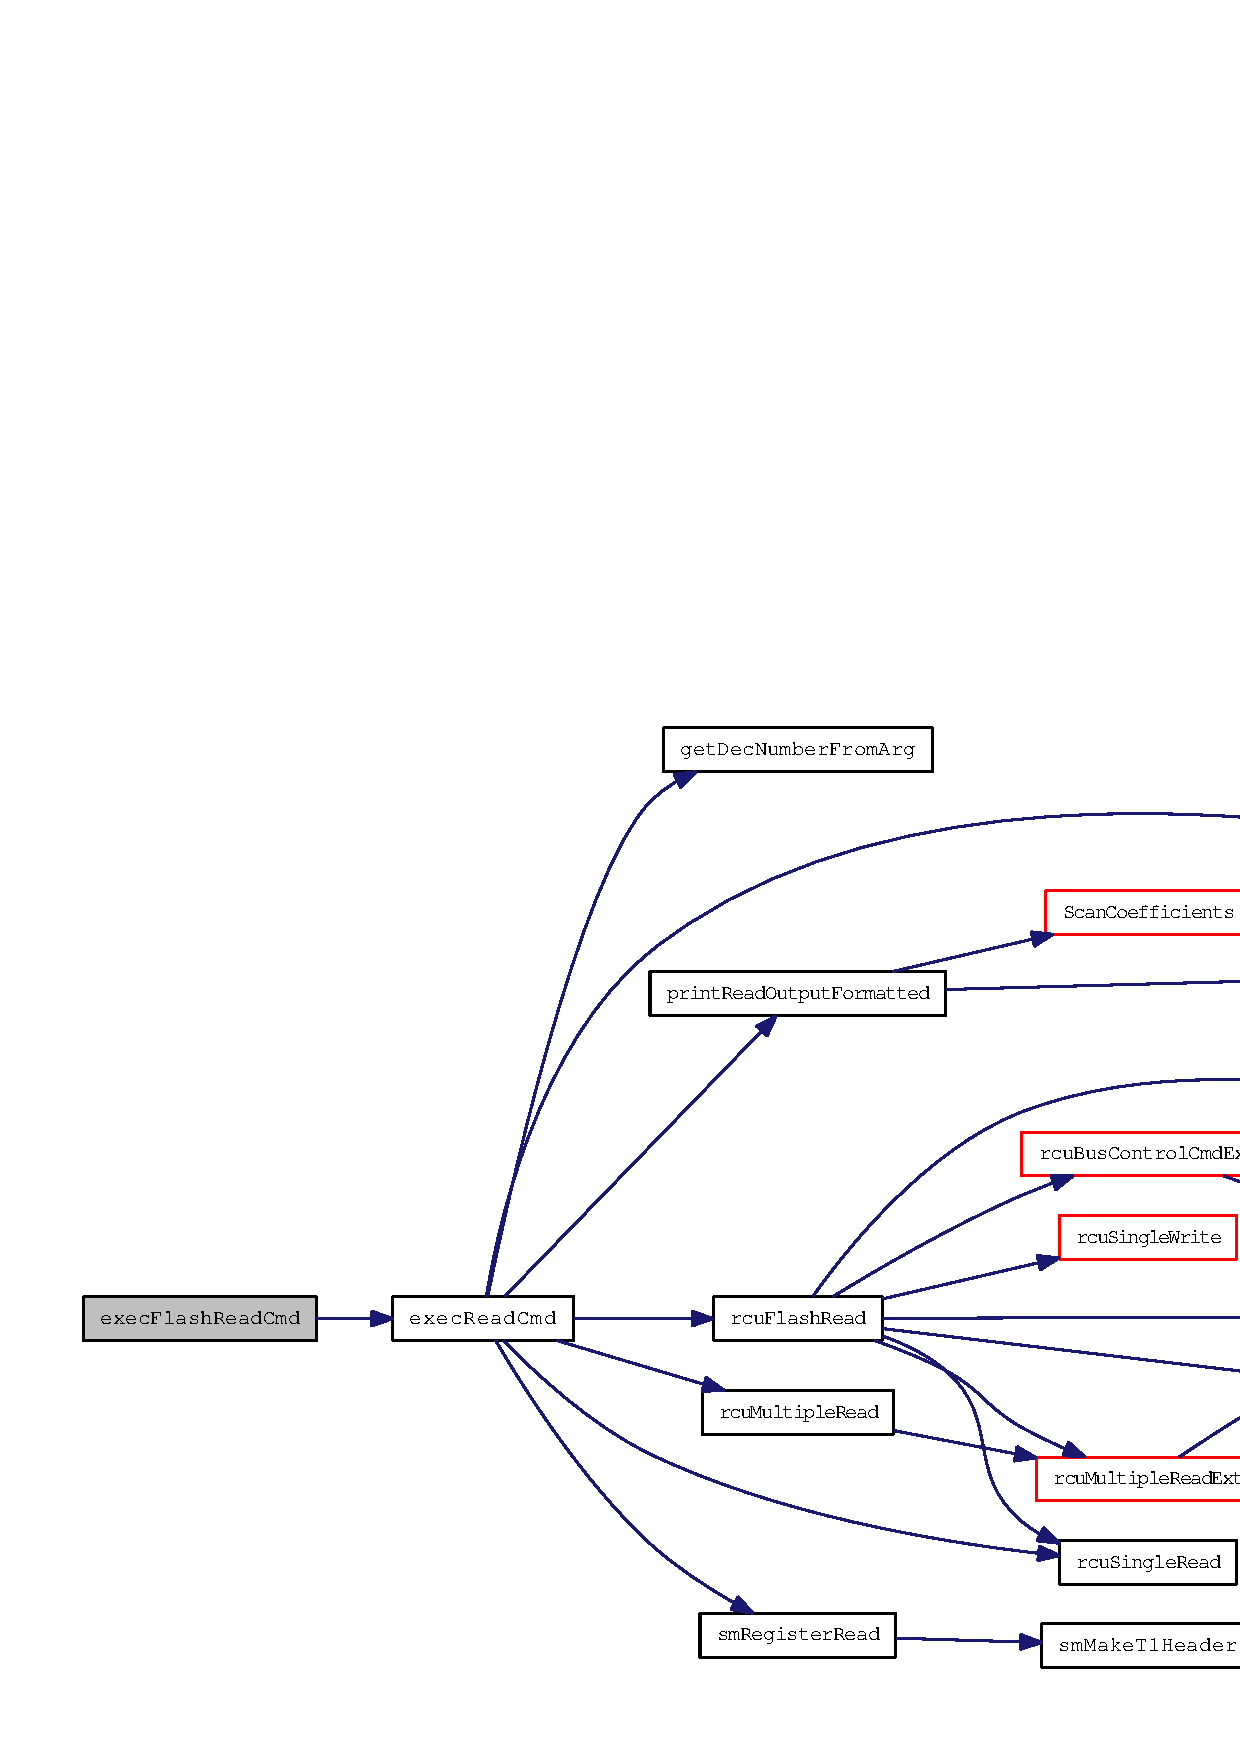
\includegraphics[width=390pt]{cmdInterpreter_8c_0069fb7612546c23d35da357dd126984_cgraph}
\end{center}
\end{figure}
\hypertarget{cmdInterpreter_8c_5df910c822508a5979806ec5d6548d65}{
\index{cmdInterpreter.c@{cmd\-Interpreter.c}!execFlashVerifyCmd@{execFlashVerifyCmd}}
\index{execFlashVerifyCmd@{execFlashVerifyCmd}!cmdInterpreter.c@{cmd\-Interpreter.c}}
\subsubsection[execFlashVerifyCmd]{\setlength{\rightskip}{0pt plus 5cm}int exec\-Flash\-Verify\-Cmd (const char $\ast$ {\em current\-Arg}, const char $\ast$$\ast$ {\em array\-Arg}, int {\em i\-Nof\-Args}, void $\ast$ {\em p\-User}, FILE $\ast$ {\em p\-Out})}}
\label{cmdInterpreter_8c_5df910c822508a5979806ec5d6548d65}




Definition at line 1704 of file cmd\-Interpreter.c.

References exec\-Write\-Cmd().

Here is the call graph for this function:\begin{figure}[H]
\begin{center}
\leavevmode
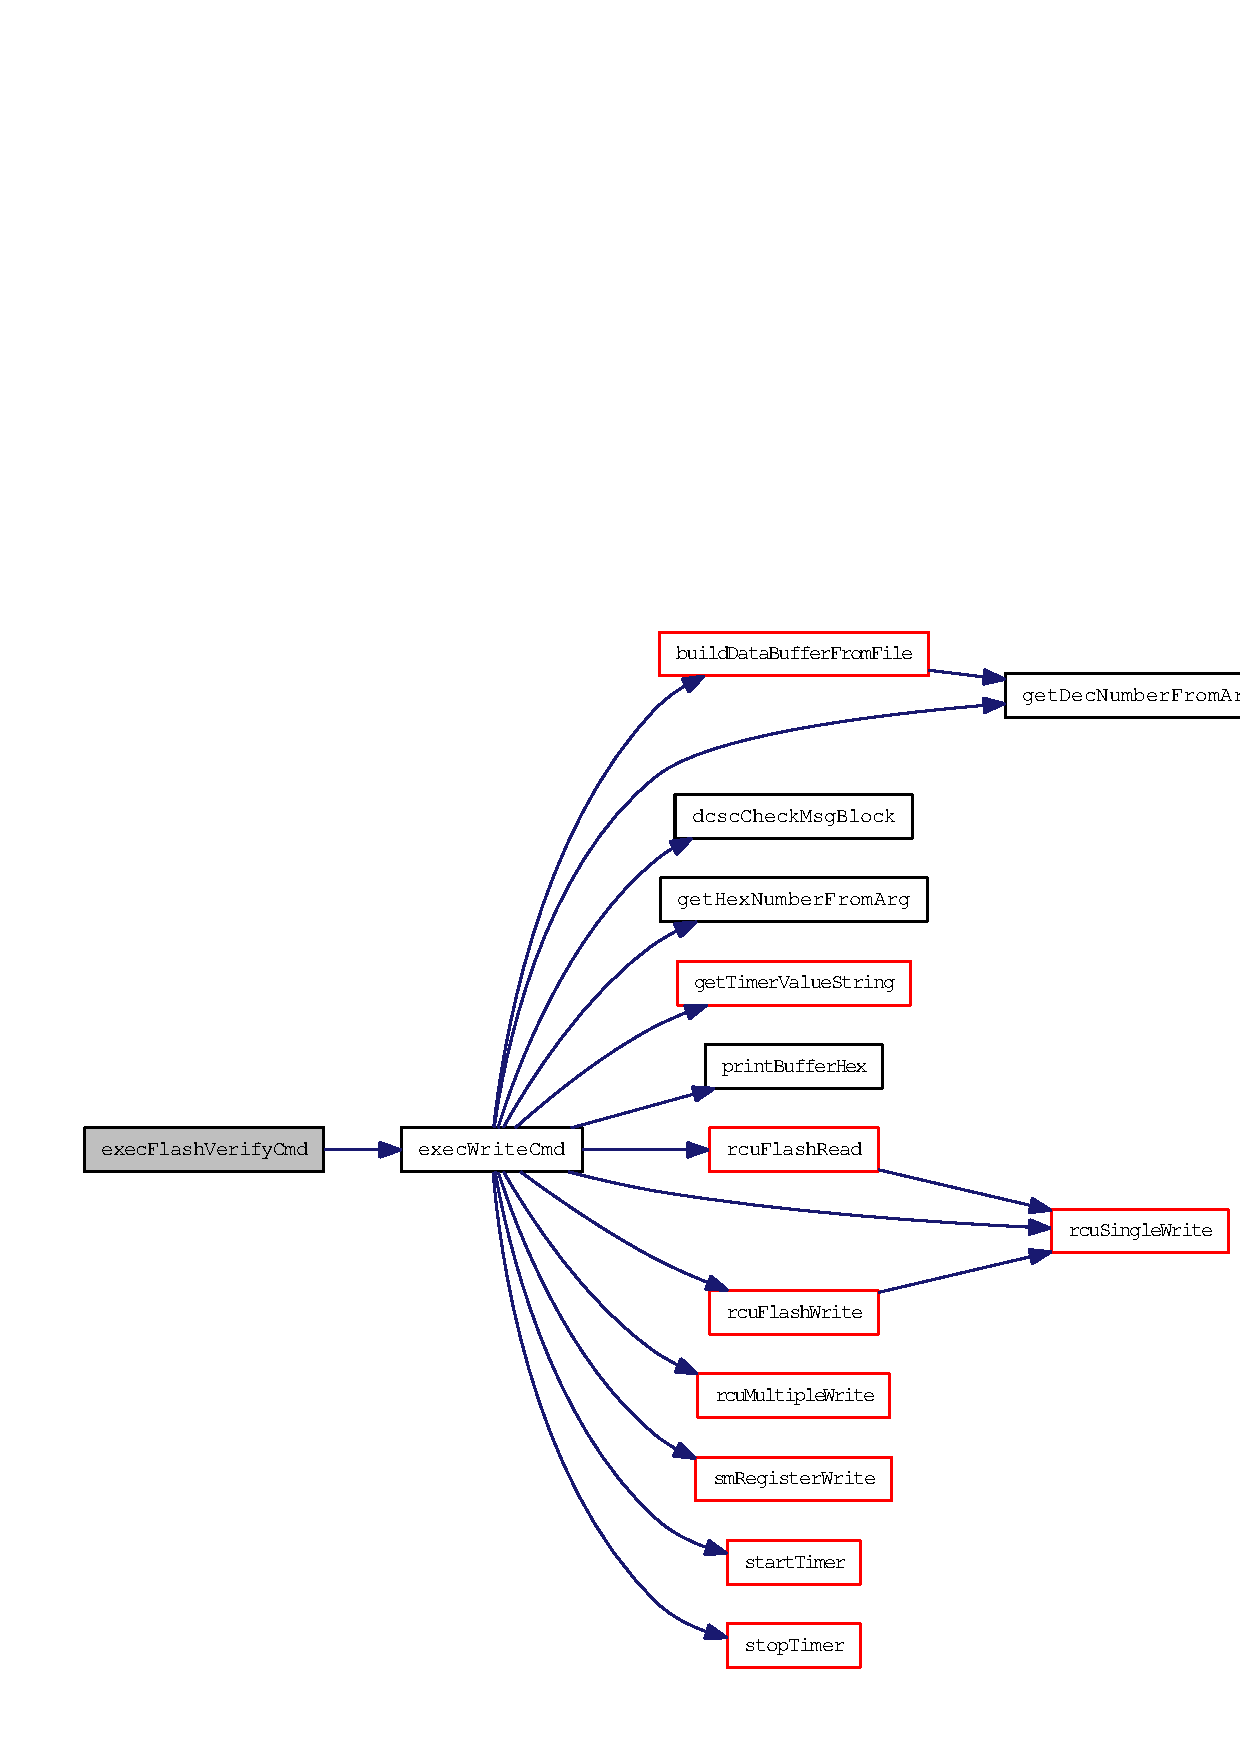
\includegraphics[width=308pt]{cmdInterpreter_8c_5df910c822508a5979806ec5d6548d65_cgraph}
\end{center}
\end{figure}
\hypertarget{cmdInterpreter_8c_765eadf200d9f408461f7469c791d22c}{
\index{cmdInterpreter.c@{cmd\-Interpreter.c}!execFlashWriteCmd@{execFlashWriteCmd}}
\index{execFlashWriteCmd@{execFlashWriteCmd}!cmdInterpreter.c@{cmd\-Interpreter.c}}
\subsubsection[execFlashWriteCmd]{\setlength{\rightskip}{0pt plus 5cm}int exec\-Flash\-Write\-Cmd (const char $\ast$ {\em current\-Arg}, const char $\ast$$\ast$ {\em array\-Arg}, int {\em i\-Nof\-Args}, void $\ast$ {\em p\-User}, FILE $\ast$ {\em p\-Out})}}
\label{cmdInterpreter_8c_765eadf200d9f408461f7469c791d22c}




Definition at line 1697 of file cmd\-Interpreter.c.

References exec\-Write\-Cmd().

Here is the call graph for this function:\begin{figure}[H]
\begin{center}
\leavevmode
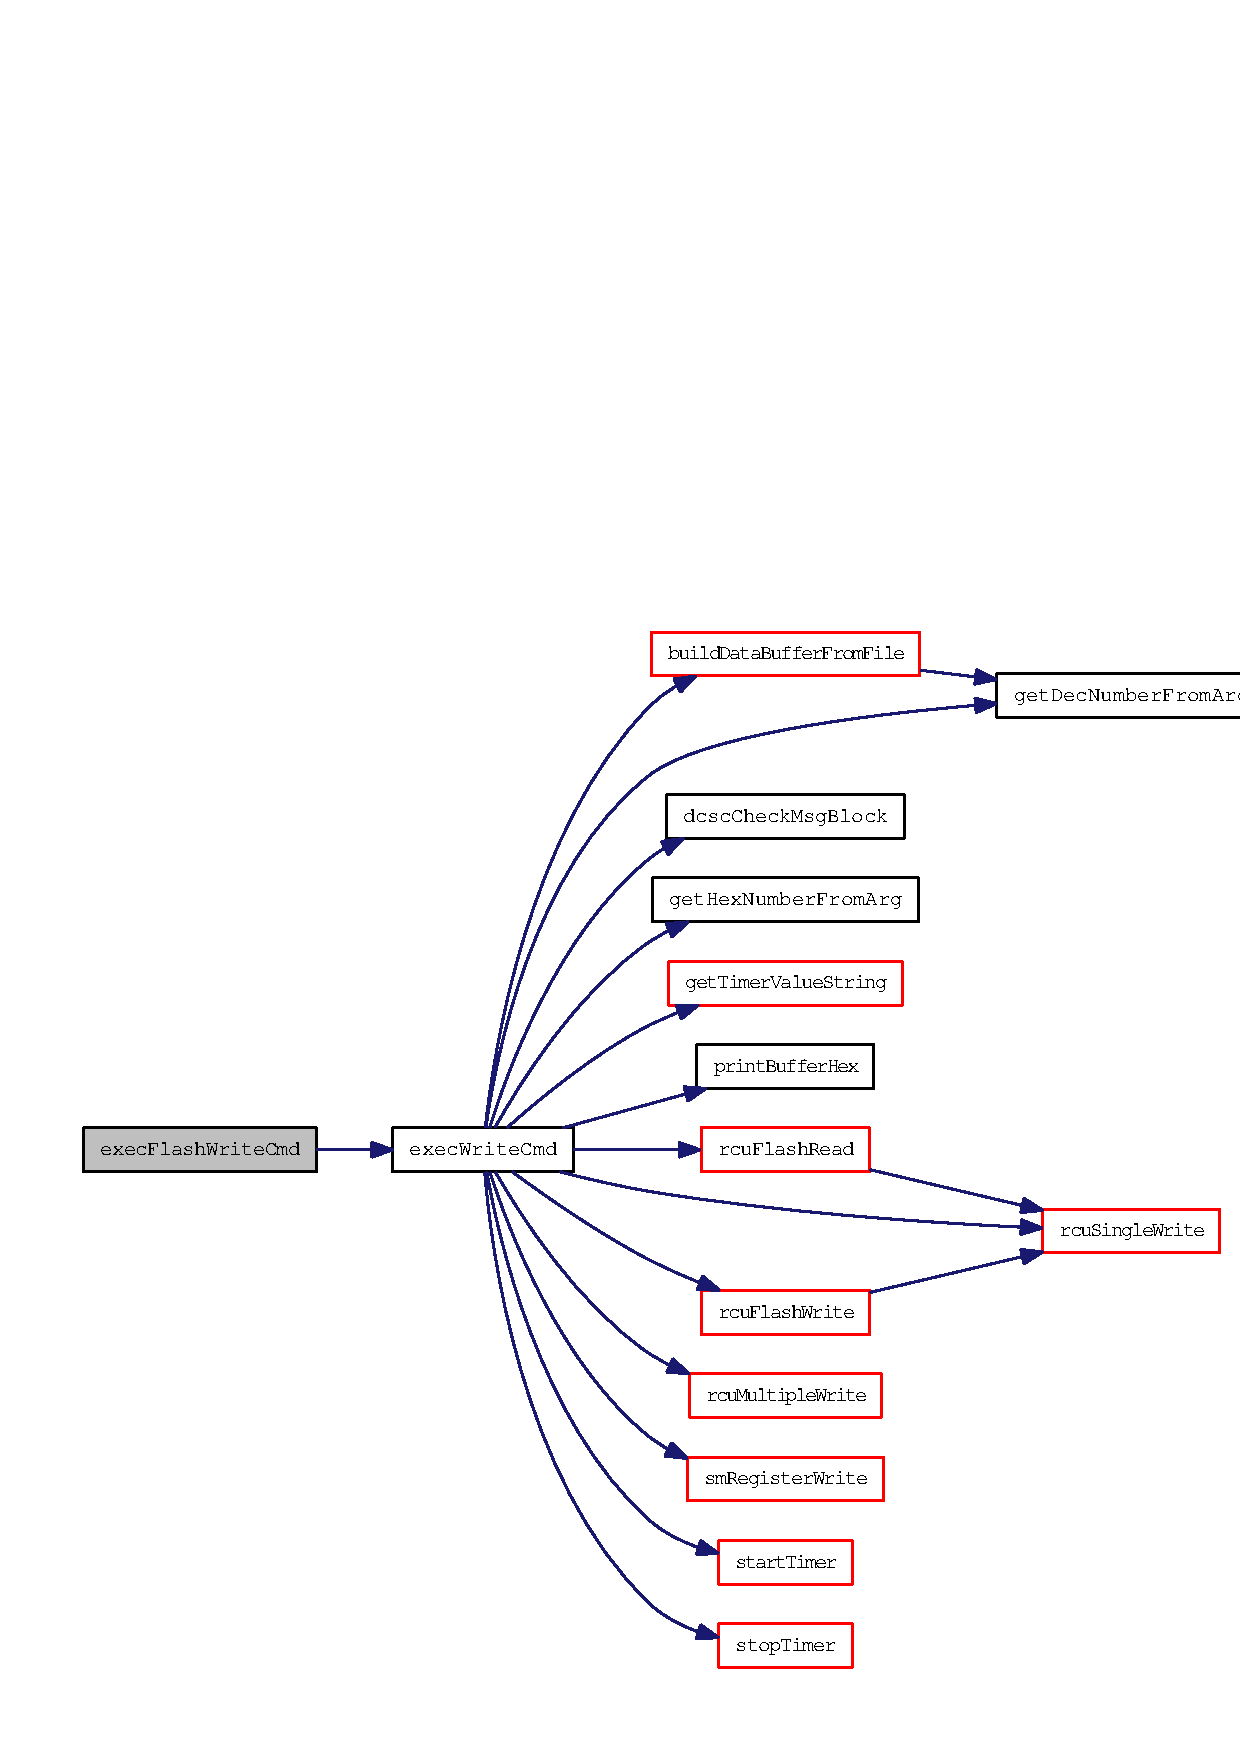
\includegraphics[width=306pt]{cmdInterpreter_8c_765eadf200d9f408461f7469c791d22c_cgraph}
\end{center}
\end{figure}
\hypertarget{cmdInterpreter_8c_a7c39db1bcd241c2ae5f259c0281abb6}{
\index{cmdInterpreter.c@{cmd\-Interpreter.c}!execReadCmd@{execReadCmd}}
\index{execReadCmd@{execReadCmd}!cmdInterpreter.c@{cmd\-Interpreter.c}}
\subsubsection[execReadCmd]{\setlength{\rightskip}{0pt plus 5cm}int exec\-Read\-Cmd (const char $\ast$$\ast$ {\em array\-Arg}, int {\em i\-Nof\-Args}, int {\em i\-Mode})}}
\label{cmdInterpreter_8c_a7c39db1bcd241c2ae5f259c0281abb6}




Definition at line 1153 of file cmd\-Interpreter.c.

References get\-Dec\-Number\-From\-Arg(), get\-Hex\-Number\-From\-Arg(), print\-Read\-Output\-Formatted(), rcu\-Flash\-Read(), rcu\-Multiple\-Read(), rcu\-Single\-Read(), and sm\-Register\-Read().

Referenced by exec\-Flash\-Read\-Cmd(), exec\-Sm\-Read\-Reg(), and execute\-Main\-Commands().

Here is the call graph for this function:\begin{figure}[H]
\begin{center}
\leavevmode
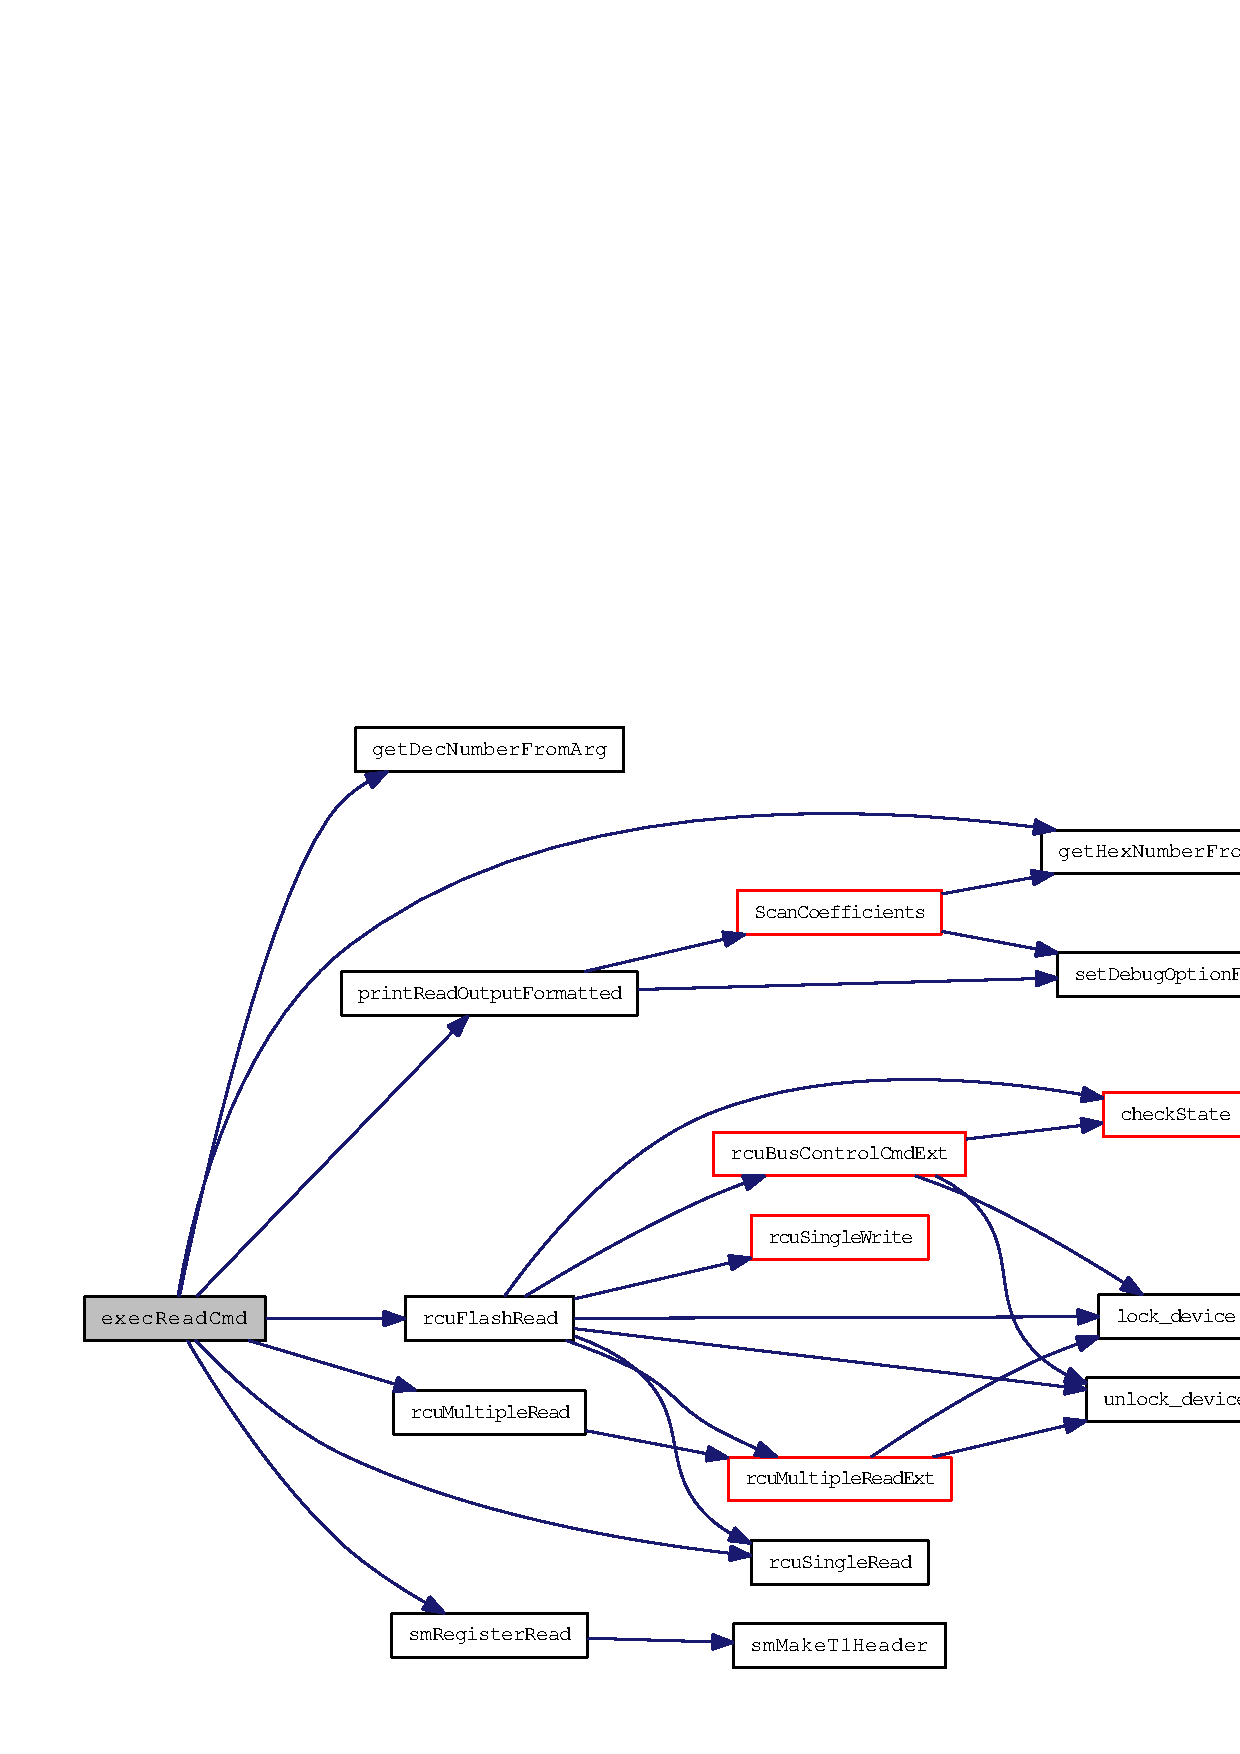
\includegraphics[width=316pt]{cmdInterpreter_8c_a7c39db1bcd241c2ae5f259c0281abb6_cgraph}
\end{center}
\end{figure}
\hypertarget{cmdInterpreter_8c_371d348f7b5d98c0ad4e7d6d20deb65c}{
\index{cmdInterpreter.c@{cmd\-Interpreter.c}!execRegReadCmd@{execRegReadCmd}}
\index{execRegReadCmd@{execRegReadCmd}!cmdInterpreter.c@{cmd\-Interpreter.c}}
\subsubsection[execRegReadCmd]{\setlength{\rightskip}{0pt plus 5cm}int exec\-Reg\-Read\-Cmd (const char $\ast$ {\em current\-Arg}, const char $\ast$$\ast$ {\em array\-Arg}, int {\em i\-Nof\-Args}, void $\ast$ {\em p\-User}, FILE $\ast$ {\em p\-Out})}}
\label{cmdInterpreter_8c_371d348f7b5d98c0ad4e7d6d20deb65c}




Definition at line 1801 of file cmd\-Interpreter.c.

References get\-Dec\-Number\-From\-Arg(), and msg\-Buf\-Read\-Register().

Here is the call graph for this function:\begin{figure}[H]
\begin{center}
\leavevmode
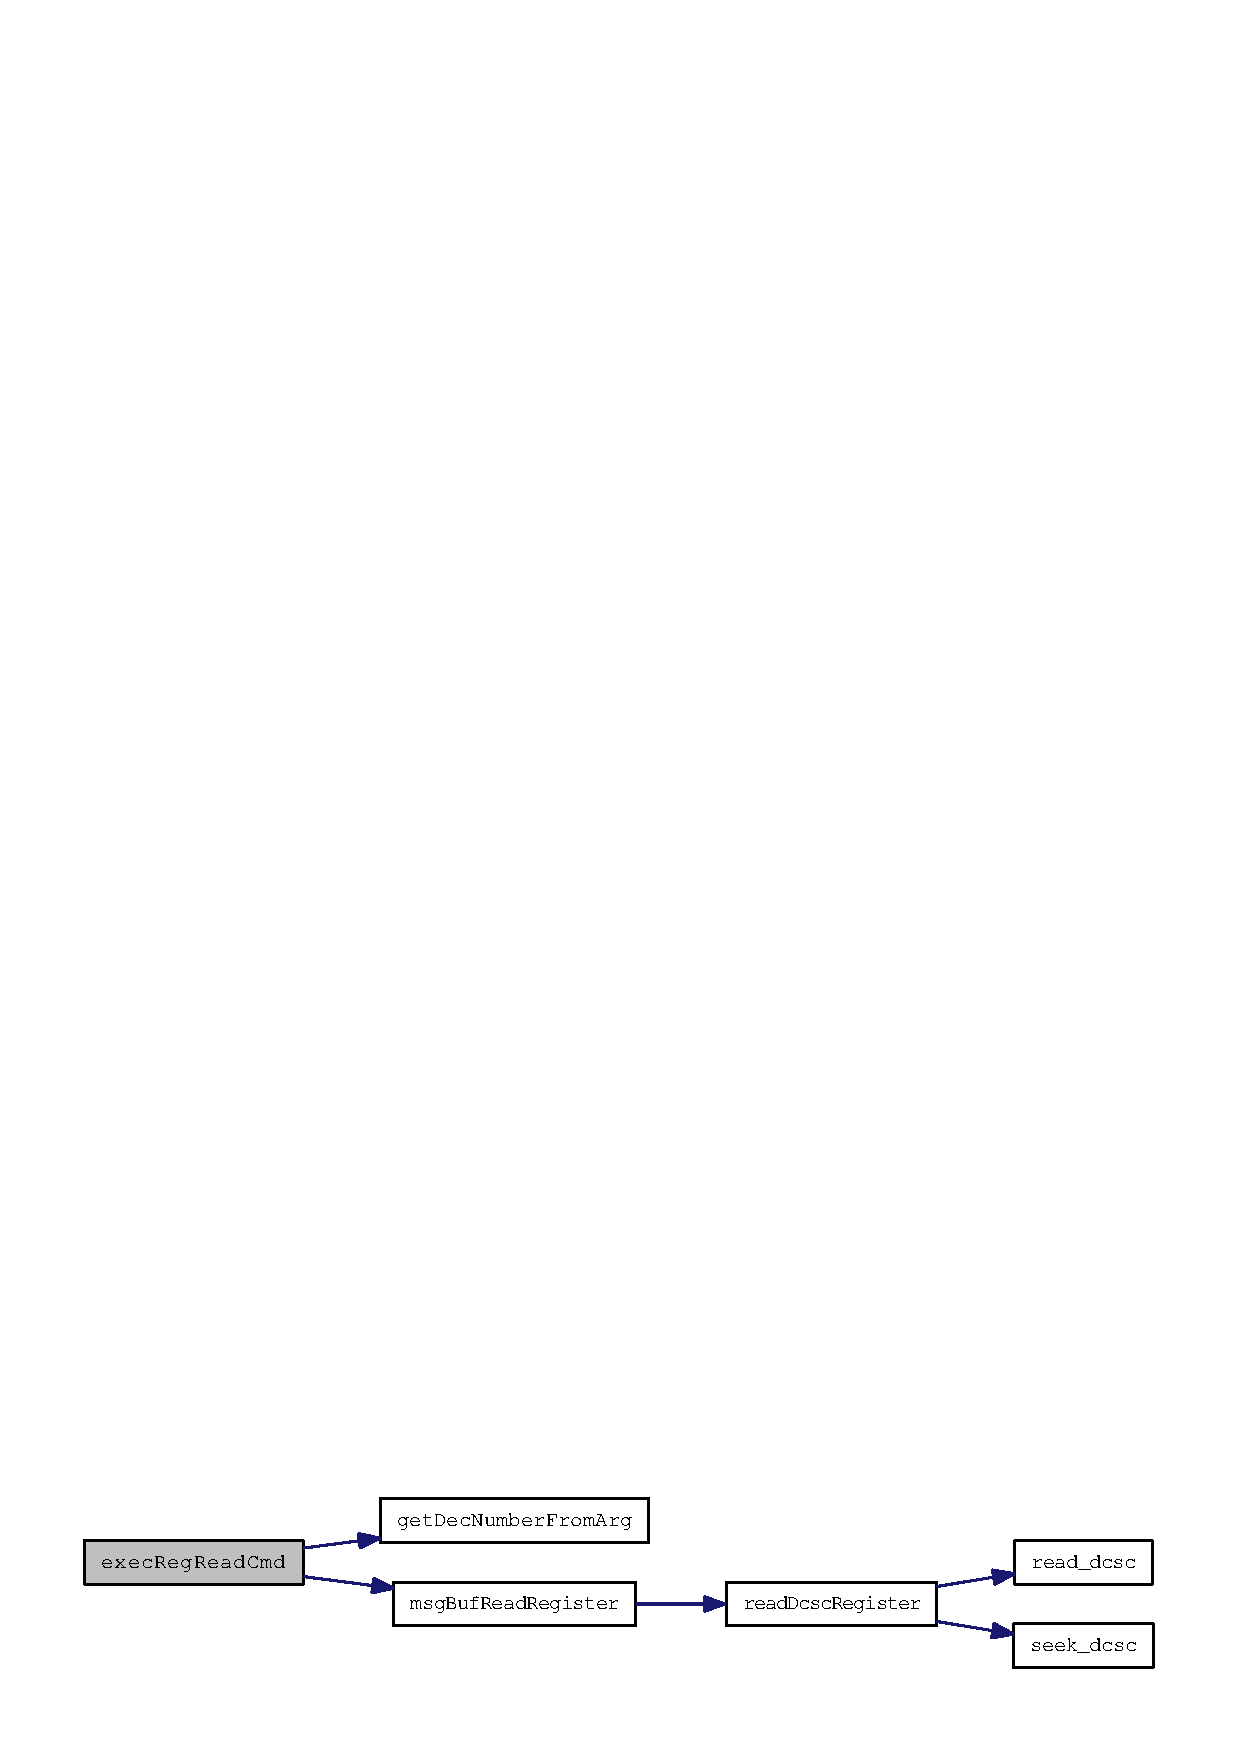
\includegraphics[width=279pt]{cmdInterpreter_8c_371d348f7b5d98c0ad4e7d6d20deb65c_cgraph}
\end{center}
\end{figure}
\hypertarget{cmdInterpreter_8c_72ffcd5a8ec94bc388af9b6d9781f5de}{
\index{cmdInterpreter.c@{cmd\-Interpreter.c}!execRegWriteCmd@{execRegWriteCmd}}
\index{execRegWriteCmd@{execRegWriteCmd}!cmdInterpreter.c@{cmd\-Interpreter.c}}
\subsubsection[execRegWriteCmd]{\setlength{\rightskip}{0pt plus 5cm}int exec\-Reg\-Write\-Cmd (const char $\ast$ {\em current\-Arg}, const char $\ast$$\ast$ {\em array\-Arg}, int {\em i\-Nof\-Args}, void $\ast$ {\em p\-User}, FILE $\ast$ {\em p\-Out})}}
\label{cmdInterpreter_8c_72ffcd5a8ec94bc388af9b6d9781f5de}




Definition at line 1785 of file cmd\-Interpreter.c.

References get\-Dec\-Number\-From\-Arg(), get\-Hex\-Number\-From\-Arg(), and msg\-Buf\-Write\-Register().

Here is the call graph for this function:\begin{figure}[H]
\begin{center}
\leavevmode
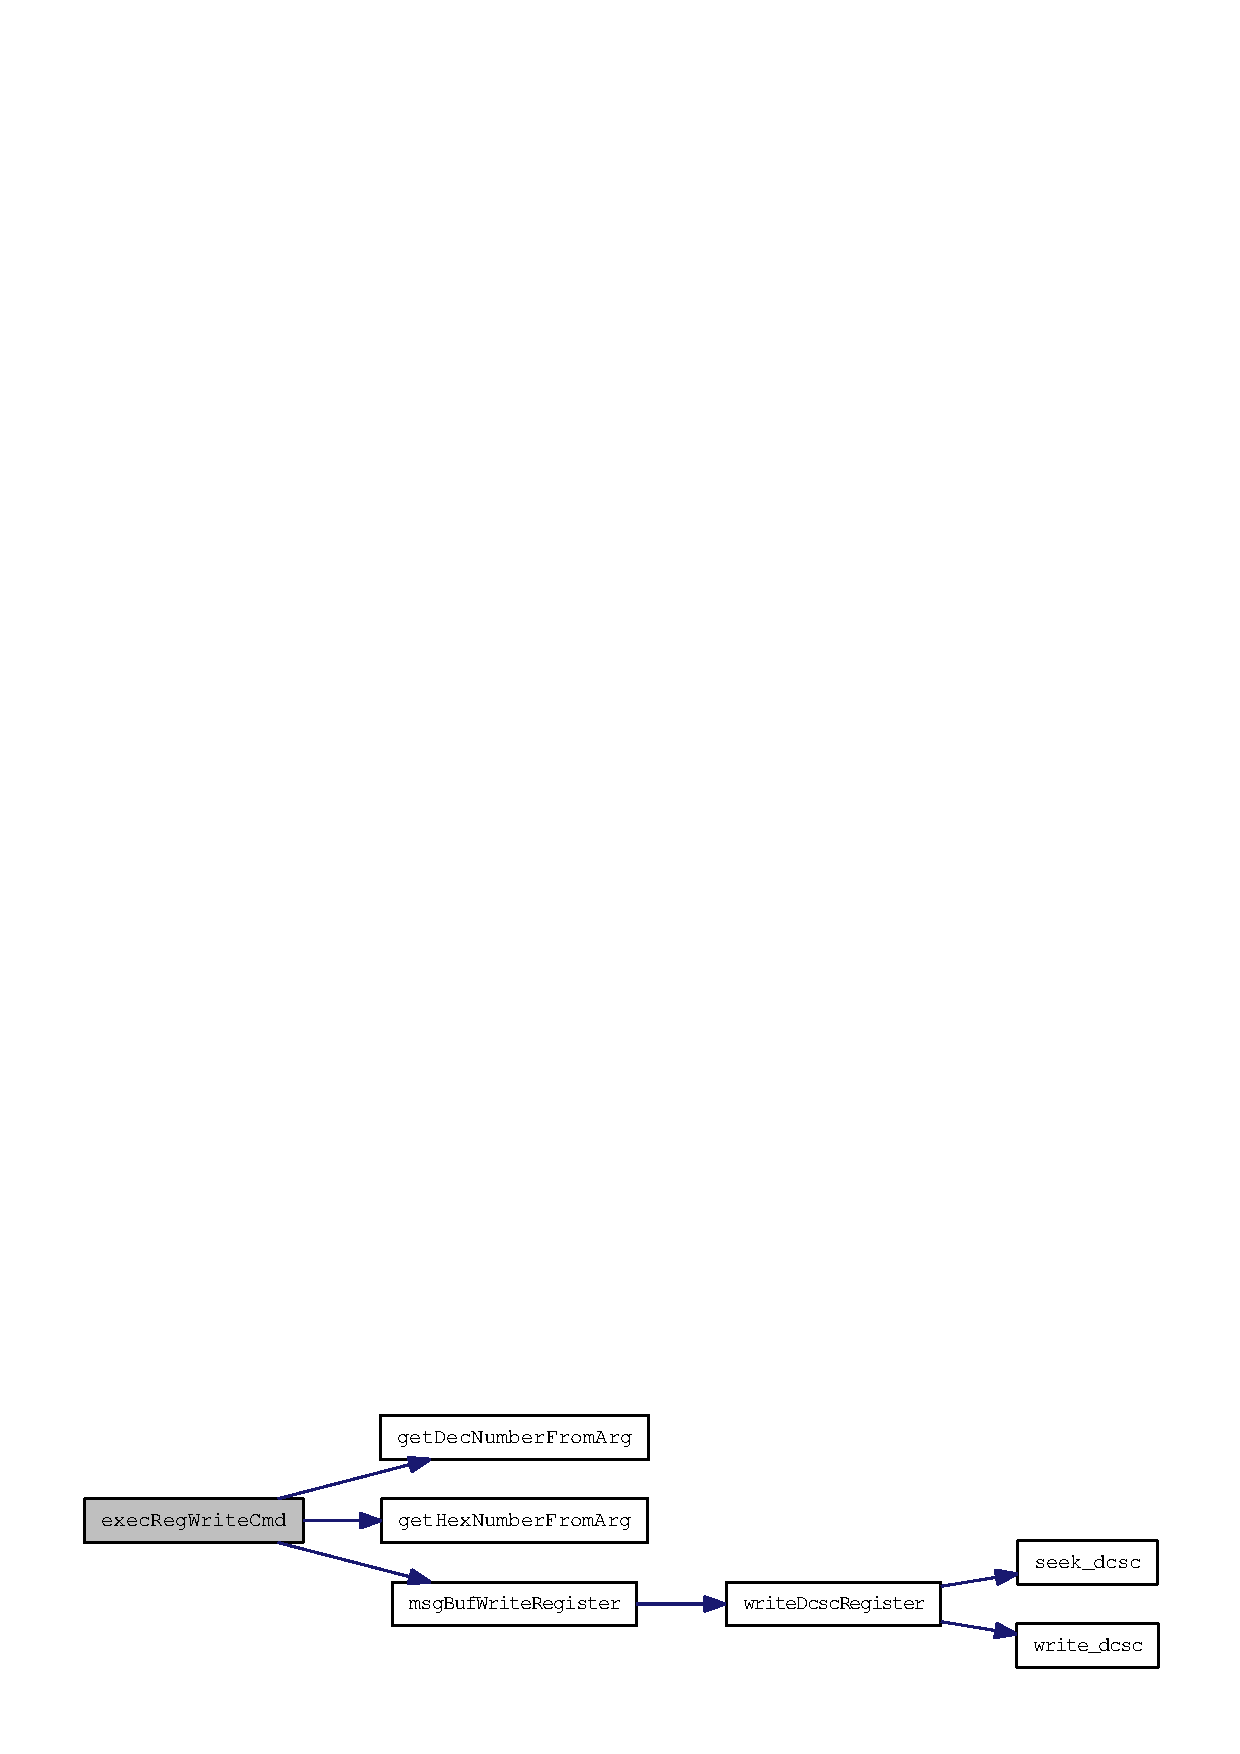
\includegraphics[width=280pt]{cmdInterpreter_8c_72ffcd5a8ec94bc388af9b6d9781f5de_cgraph}
\end{center}
\end{figure}
\hypertarget{cmdInterpreter_8c_acf8d85528167524bef8a5e23b9ffd99}{
\index{cmdInterpreter.c@{cmd\-Interpreter.c}!execSmReadReg@{execSmReadReg}}
\index{execSmReadReg@{execSmReadReg}!cmdInterpreter.c@{cmd\-Interpreter.c}}
\subsubsection[execSmReadReg]{\setlength{\rightskip}{0pt plus 5cm}int exec\-Sm\-Read\-Reg (const char $\ast$ {\em current\-Arg}, const char $\ast$$\ast$ {\em array\-Arg}, int {\em i\-Nof\-Args}, void $\ast$ {\em p\-User}, FILE $\ast$ {\em p\-Out})}}
\label{cmdInterpreter_8c_acf8d85528167524bef8a5e23b9ffd99}




Definition at line 1753 of file cmd\-Interpreter.c.

References exec\-Read\-Cmd().

Here is the call graph for this function:\begin{figure}[H]
\begin{center}
\leavevmode
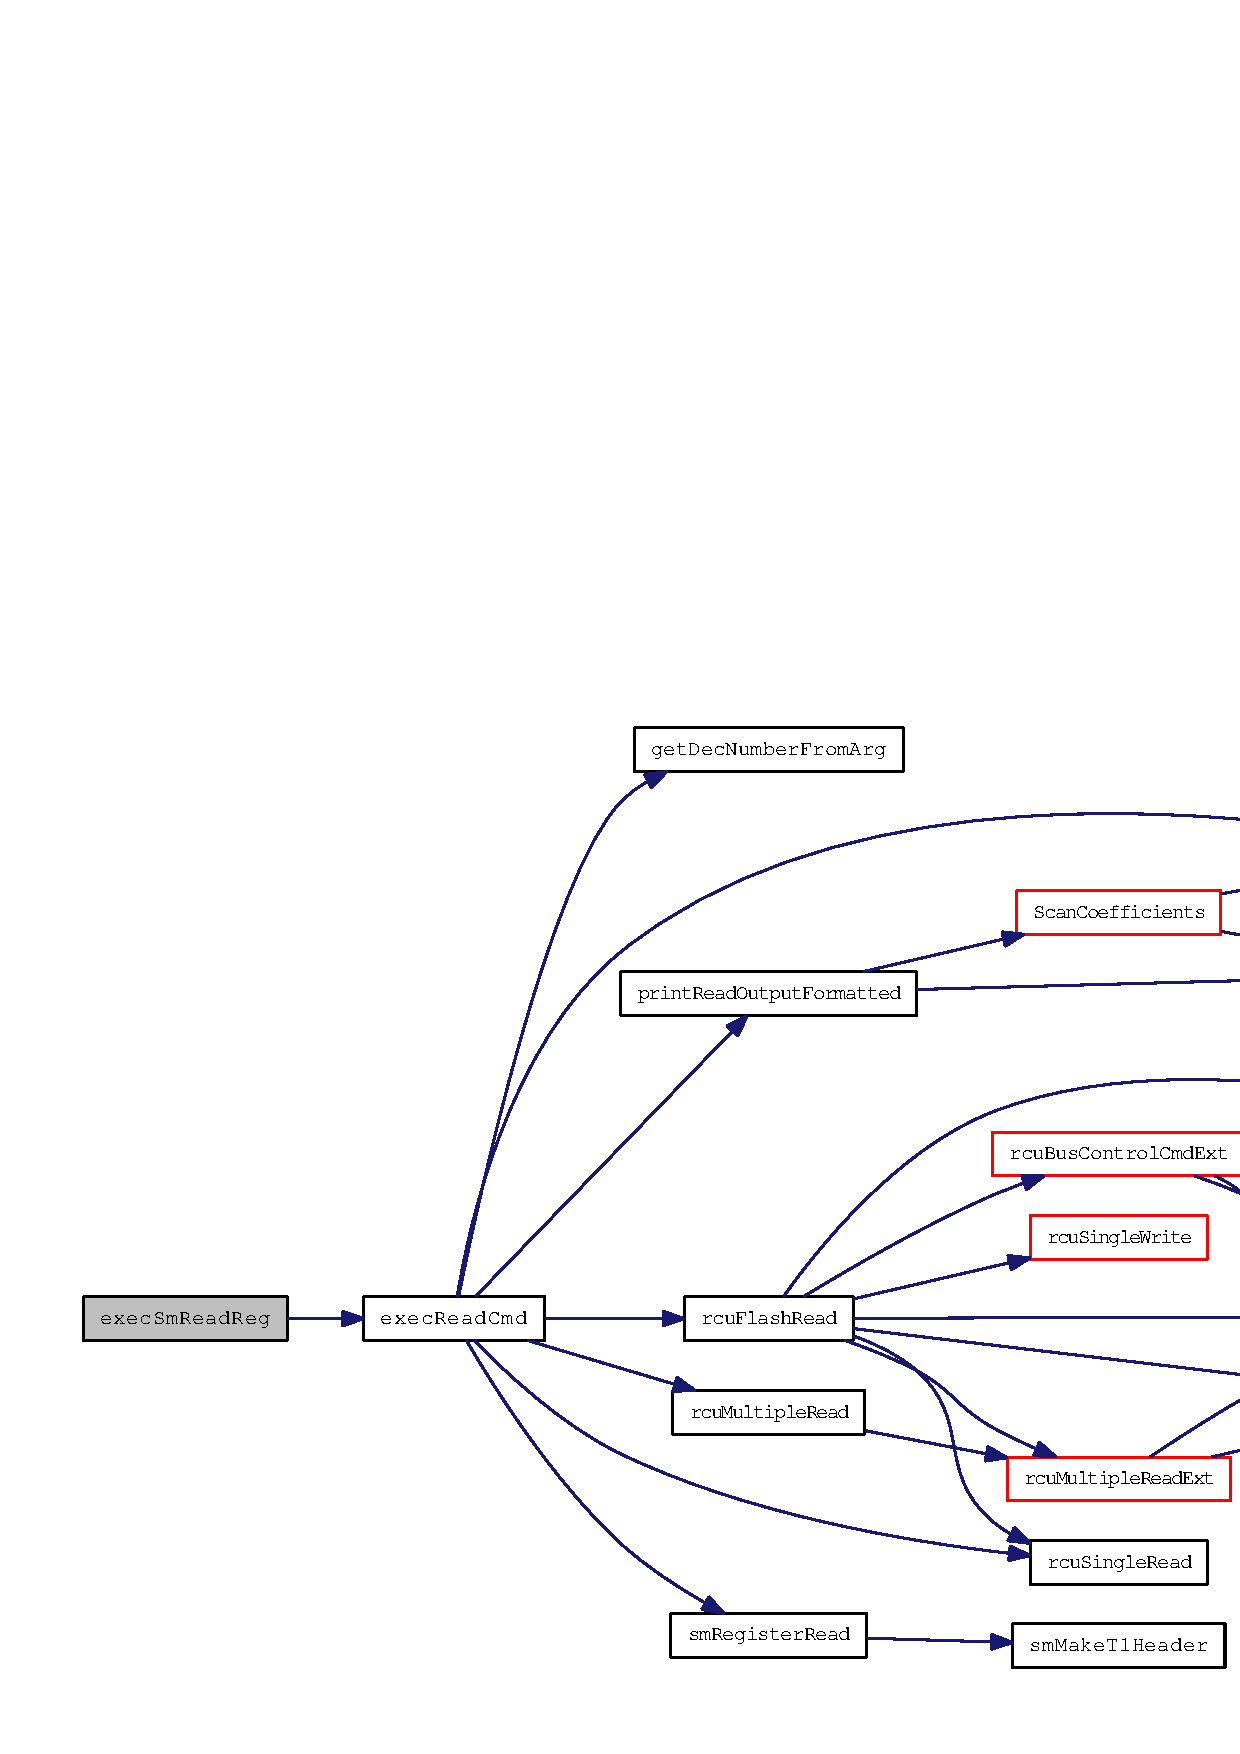
\includegraphics[width=383pt]{cmdInterpreter_8c_acf8d85528167524bef8a5e23b9ffd99_cgraph}
\end{center}
\end{figure}
\hypertarget{cmdInterpreter_8c_a8f5aca148fba0272ac3acfee150f651}{
\index{cmdInterpreter.c@{cmd\-Interpreter.c}!execSmWriteReg@{execSmWriteReg}}
\index{execSmWriteReg@{execSmWriteReg}!cmdInterpreter.c@{cmd\-Interpreter.c}}
\subsubsection[execSmWriteReg]{\setlength{\rightskip}{0pt plus 5cm}int exec\-Sm\-Write\-Reg (const char $\ast$ {\em current\-Arg}, const char $\ast$$\ast$ {\em array\-Arg}, int {\em i\-Nof\-Args}, void $\ast$ {\em p\-User}, FILE $\ast$ {\em p\-Out})}}
\label{cmdInterpreter_8c_a8f5aca148fba0272ac3acfee150f651}




Definition at line 1746 of file cmd\-Interpreter.c.

References exec\-Write\-Cmd().

Here is the call graph for this function:\begin{figure}[H]
\begin{center}
\leavevmode
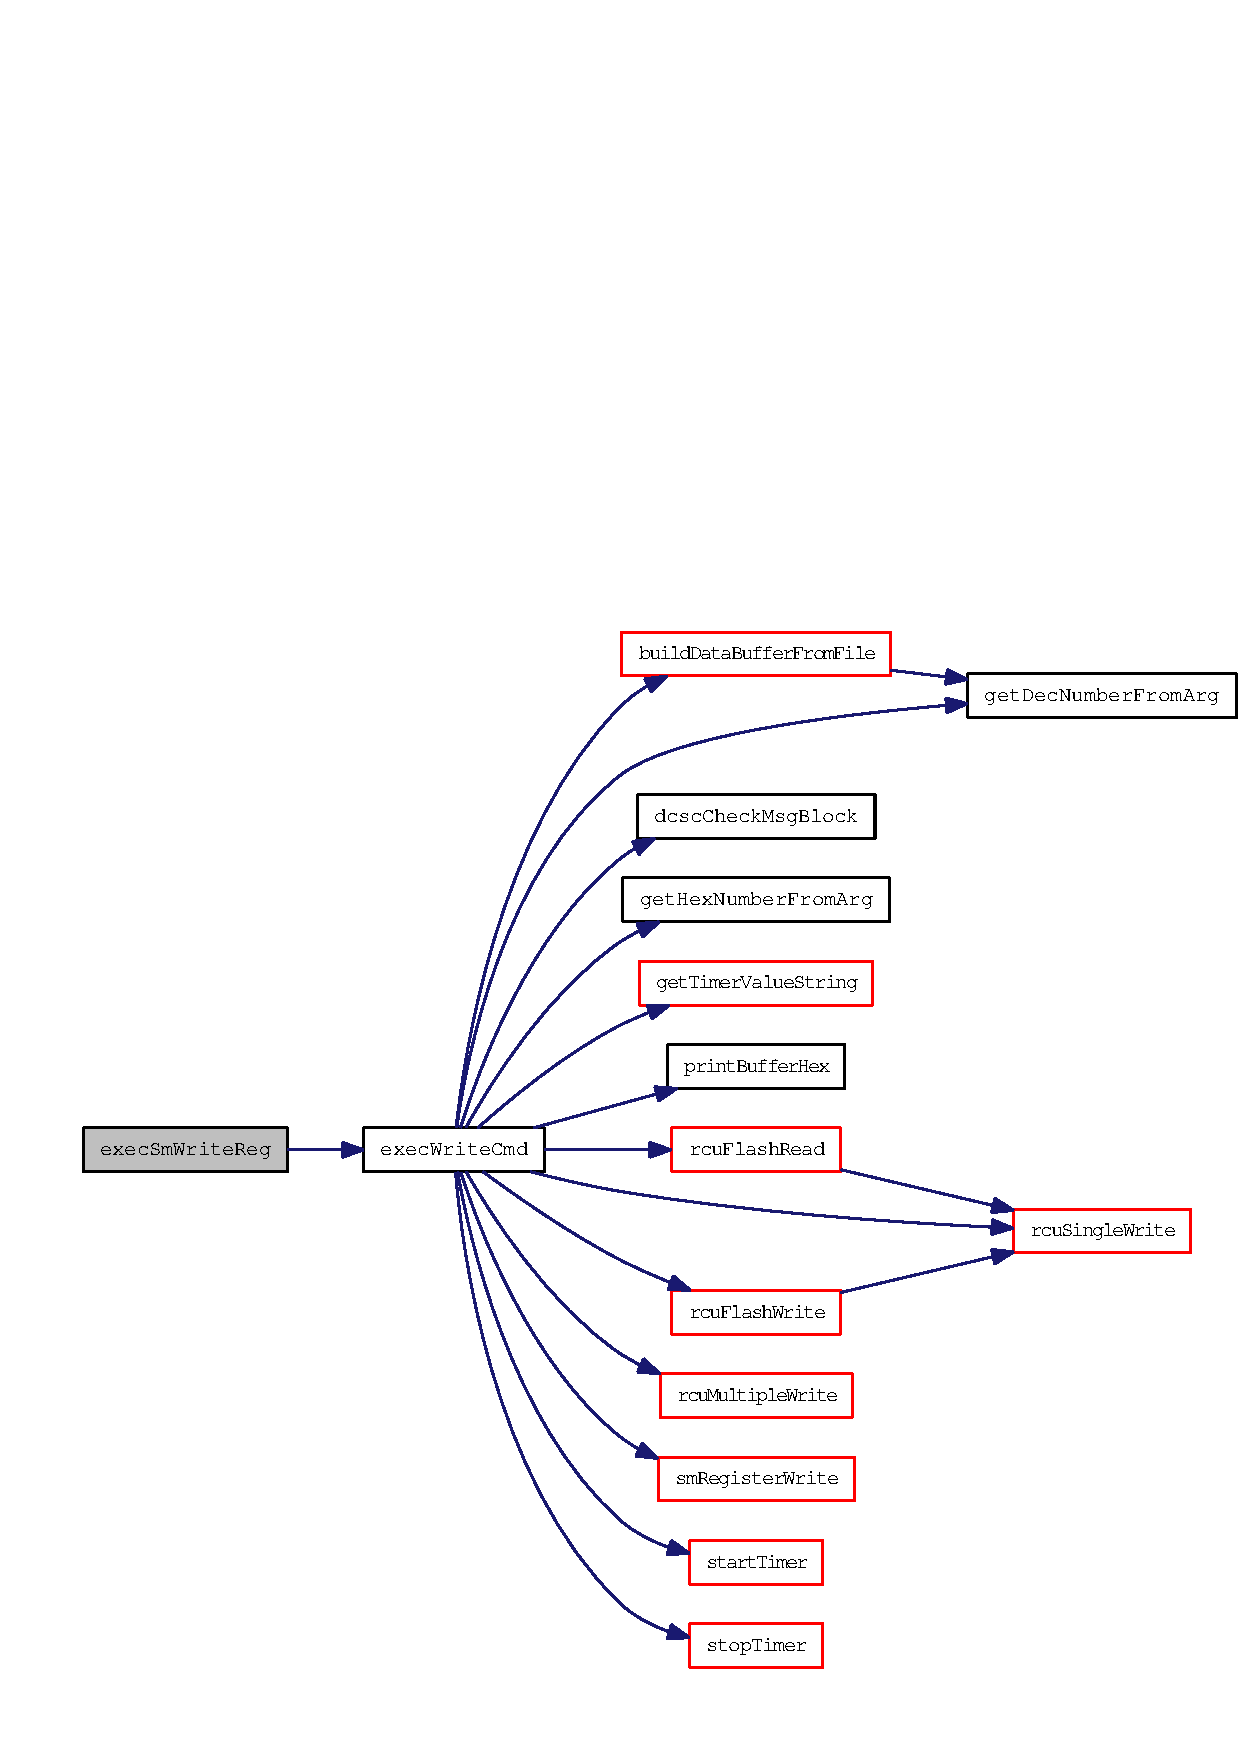
\includegraphics[width=299pt]{cmdInterpreter_8c_a8f5aca148fba0272ac3acfee150f651_cgraph}
\end{center}
\end{figure}
\hypertarget{cmdInterpreter_8c_54cbd6e4f4a91310f0c408dc5c6b413d}{
\index{cmdInterpreter.c@{cmd\-Interpreter.c}!executeCommandArgs@{executeCommandArgs}}
\index{executeCommandArgs@{executeCommandArgs}!cmdInterpreter.c@{cmd\-Interpreter.c}}
\subsubsection[executeCommandArgs]{\setlength{\rightskip}{0pt plus 5cm}int execute\-Command\-Args (int {\em i\-Nof\-Args}, const char $\ast$$\ast$ {\em array\-Arg})}}
\label{cmdInterpreter_8c_54cbd6e4f4a91310f0c408dc5c6b413d}




Definition at line 1892 of file cmd\-Interpreter.c.

References main\-Commands, mr\-Shell\-Prim\-Clone\-Def(), and Scan\-Arguments().

Referenced by execute\-Command\-Line(), and main().

Here is the call graph for this function:\begin{figure}[H]
\begin{center}
\leavevmode
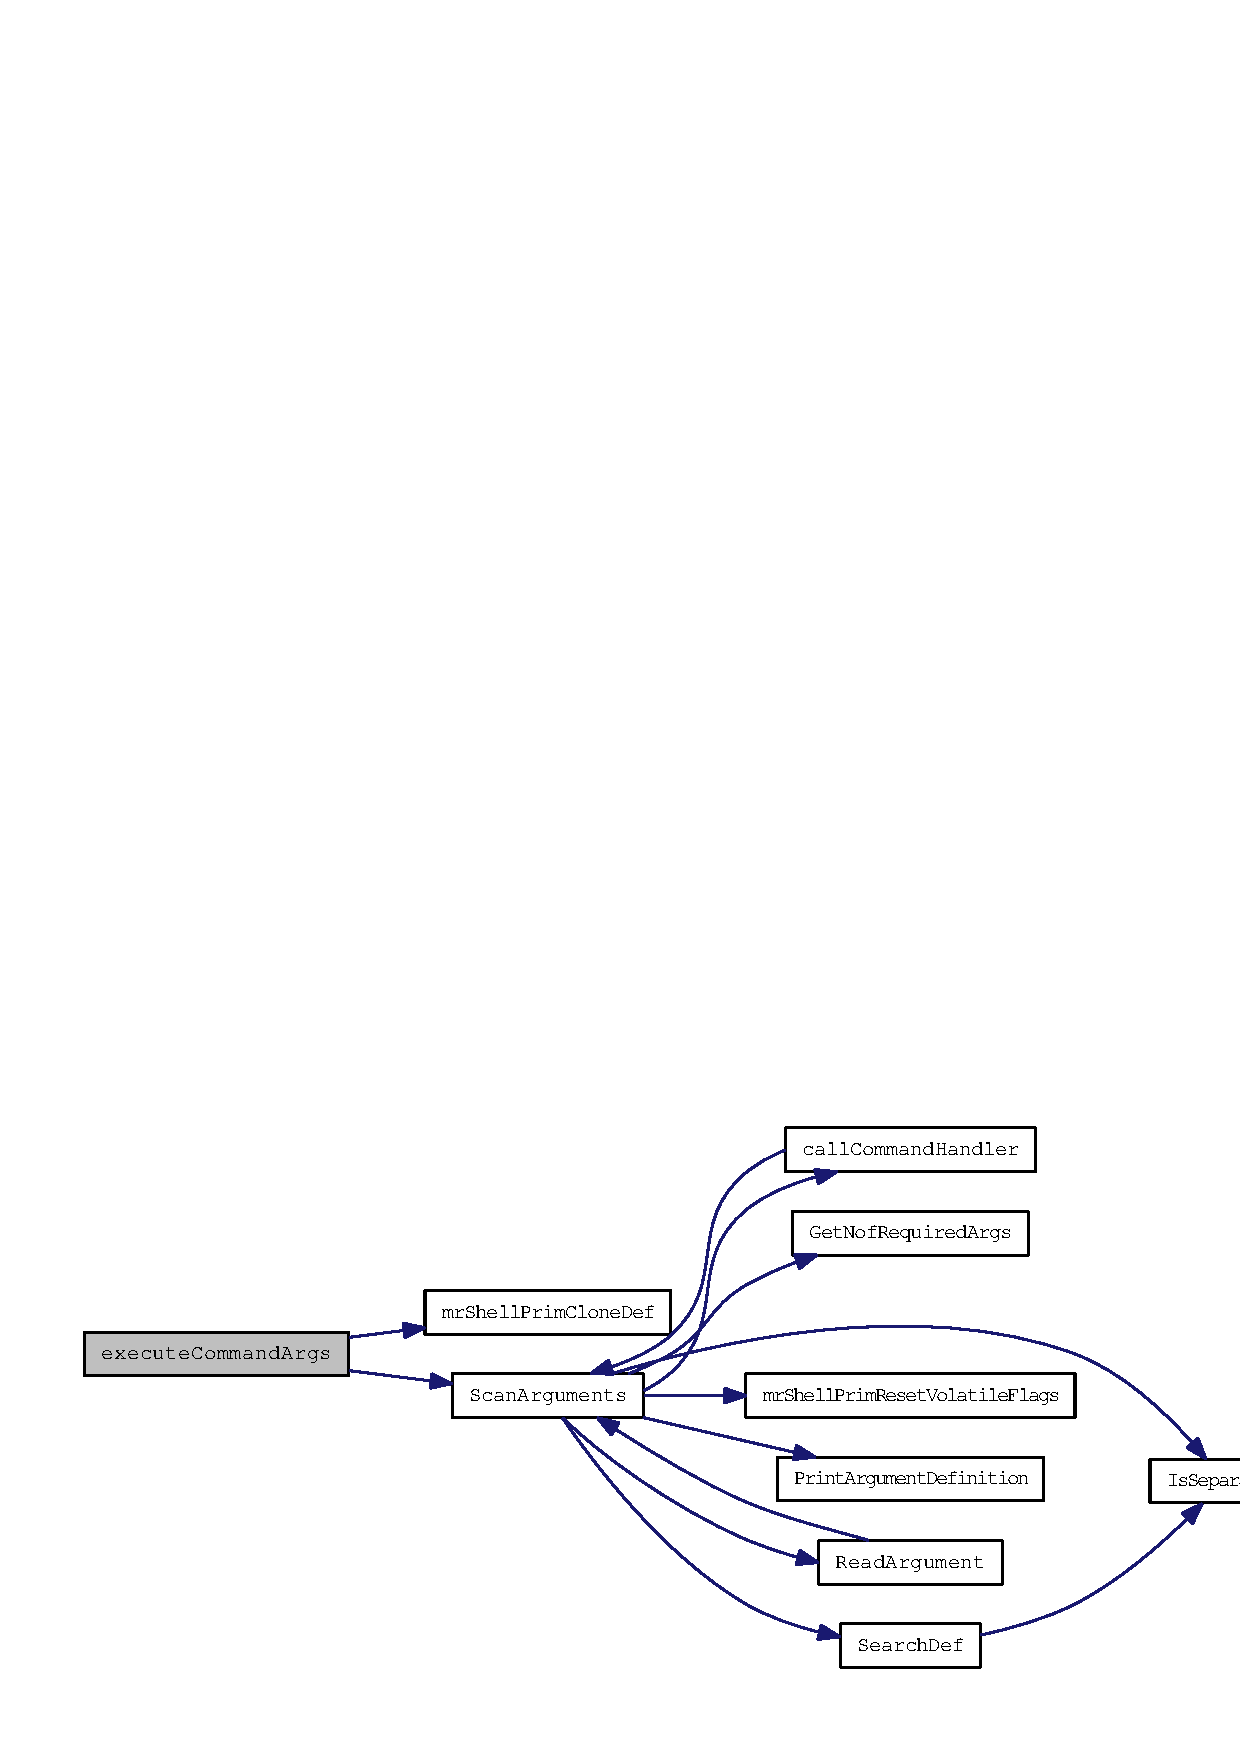
\includegraphics[width=313pt]{cmdInterpreter_8c_54cbd6e4f4a91310f0c408dc5c6b413d_cgraph}
\end{center}
\end{figure}
\hypertarget{cmdInterpreter_8c_48086998882e7d163126de4100aa12ac}{
\index{cmdInterpreter.c@{cmd\-Interpreter.c}!executeCommandLine@{executeCommandLine}}
\index{executeCommandLine@{executeCommandLine}!cmdInterpreter.c@{cmd\-Interpreter.c}}
\subsubsection[executeCommandLine]{\setlength{\rightskip}{0pt plus 5cm}int execute\-Command\-Line (char $\ast$ {\em p\-Cmd\-Line})}}
\label{cmdInterpreter_8c_48086998882e7d163126de4100aa12ac}




Definition at line 1904 of file cmd\-Interpreter.c.

References build\-Arguments\-From\-Command\-Line(), DBG\_\-ARGUMENT\_\-CONVERT, execute\-Command\-Args(), and set\-Debug\-Option\-Flag().

Referenced by exec\-Batch(), and main().

Here is the call graph for this function:\begin{figure}[H]
\begin{center}
\leavevmode
\includegraphics[width=273pt]{cmdInterpreter_8c_48086998882e7d163126de4100aa12ac_cgraph}
\end{center}
\end{figure}
\hypertarget{cmdInterpreter_8c_11ec76f8e60016409f2f33d10c70ef7e}{
\index{cmdInterpreter.c@{cmd\-Interpreter.c}!executeMainCommands@{executeMainCommands}}
\index{executeMainCommands@{executeMainCommands}!cmdInterpreter.c@{cmd\-Interpreter.c}}
\subsubsection[executeMainCommands]{\setlength{\rightskip}{0pt plus 5cm}int execute\-Main\-Commands (const char $\ast$ {\em current\-Arg}, const char $\ast$$\ast$ {\em array\-Arg}, int {\em i\-Nof\-Args}, void $\ast$ {\em p\-User}, FILE $\ast$ {\em p\-Out})}}
\label{cmdInterpreter_8c_11ec76f8e60016409f2f33d10c70ef7e}




Definition at line 1459 of file cmd\-Interpreter.c.

References clear\-Debug\-Option\-Flag(), clear\-MRTimer\-Debug\-Flag(), CMD\_\-STRING\_\-MRT\_\-DEBUG, CMD\_\-STRING\_\-PROFILE, DBG\_\-ARGUMENT\_\-CONVERT, DBG\_\-DEFAULT, exec\-Batch(), exec\-Read\-Cmd(), exec\-Write\-Cmd(), g\_\-profiling, get\-Dec\-Number\-From\-Arg(), get\-Hex\-Number\-From\-Arg(), print\-Batch\-Proc\-Help(), print\-Debug\-Help(), print\-Help(), print\-Read\-Help(), read\-Time(), set\-Debug\-Option\-Flag(), set\-Debug\-Options(), set\-MRTimer\-Debug\-Flag(), timed\-Wait(), and wait\-Condition().

Here is the call graph for this function:\begin{figure}[H]
\begin{center}
\leavevmode
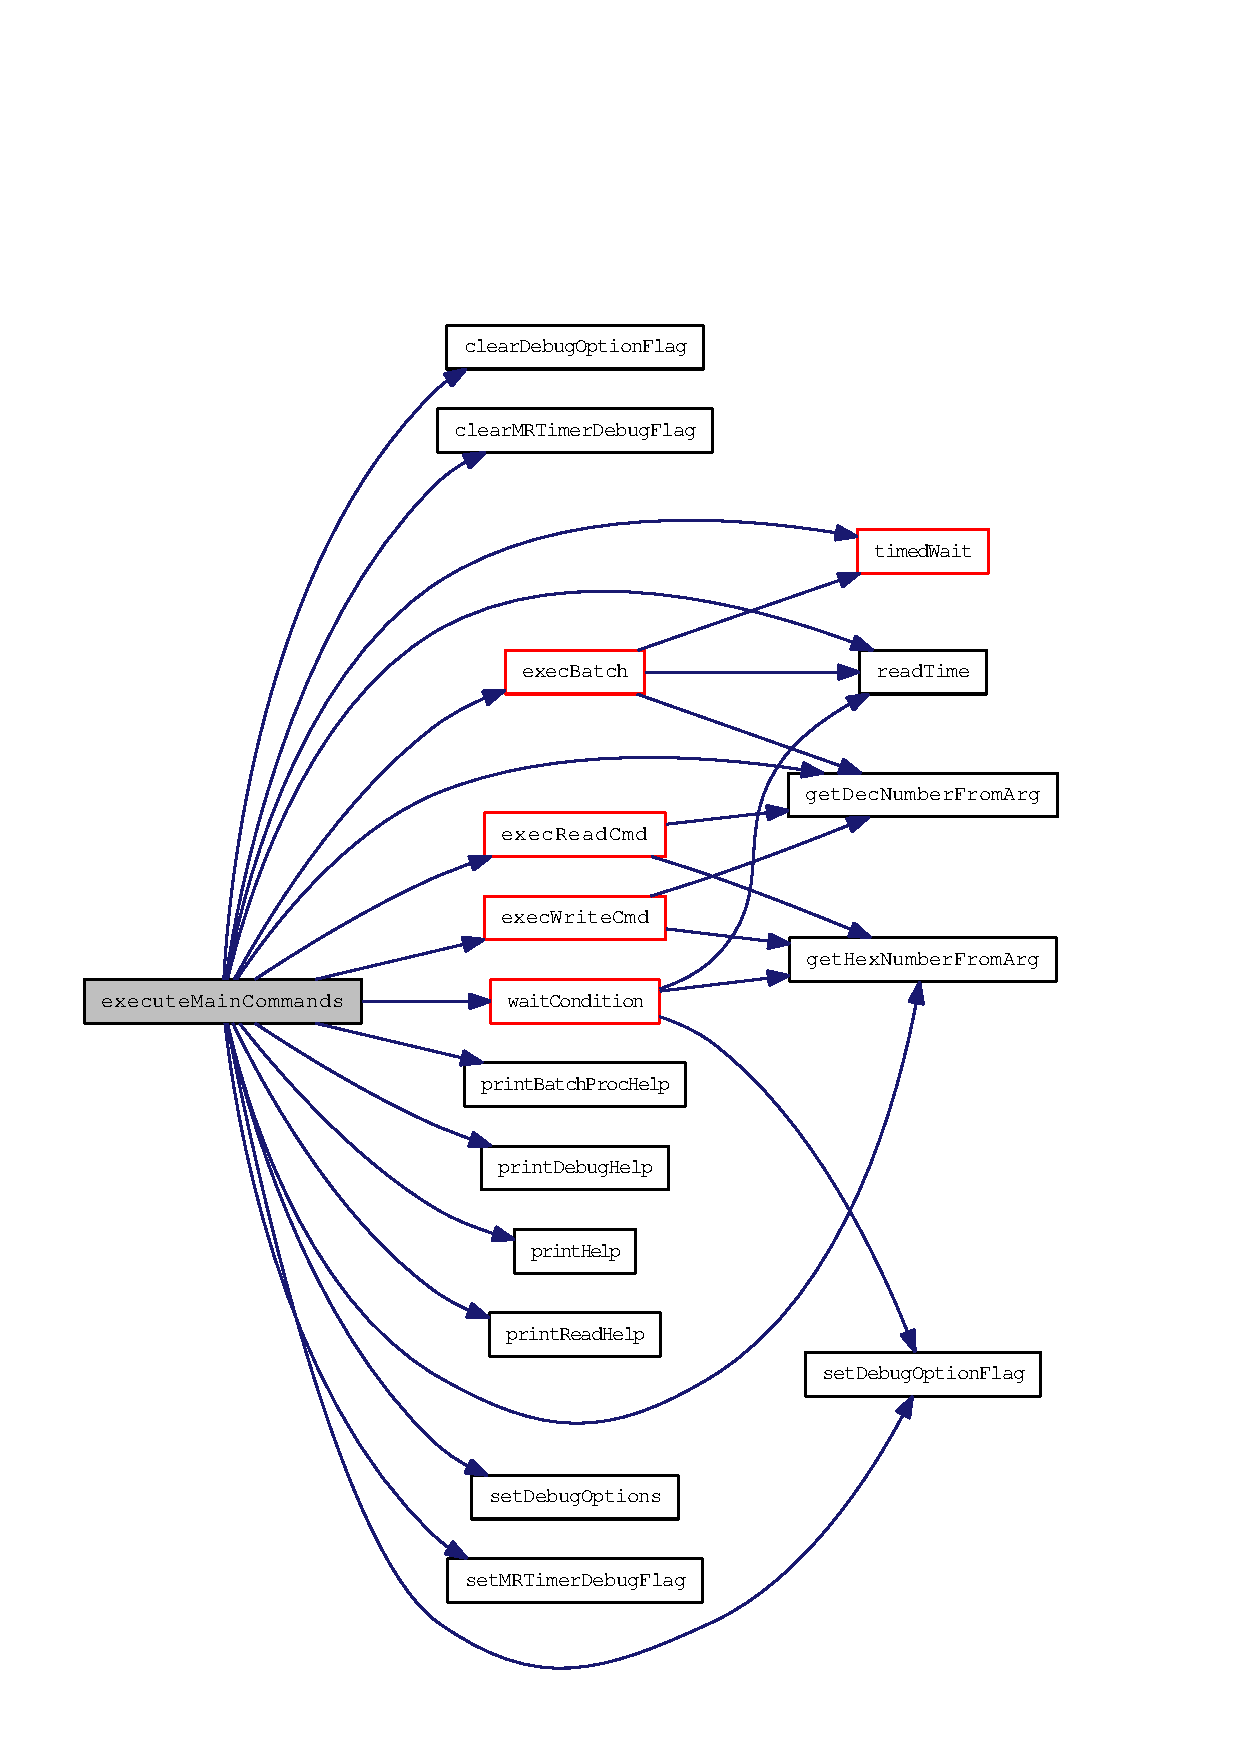
\includegraphics[width=256pt]{cmdInterpreter_8c_11ec76f8e60016409f2f33d10c70ef7e_cgraph}
\end{center}
\end{figure}
\hypertarget{cmdInterpreter_8c_6f67c6327e24c23440e0fdf83d06e41d}{
\index{cmdInterpreter.c@{cmd\-Interpreter.c}!execWriteCmd@{execWriteCmd}}
\index{execWriteCmd@{execWriteCmd}!cmdInterpreter.c@{cmd\-Interpreter.c}}
\subsubsection[execWriteCmd]{\setlength{\rightskip}{0pt plus 5cm}int exec\-Write\-Cmd (const char $\ast$$\ast$ {\em array\-Arg}, int {\em i\-Nof\-Args}, int {\em i\-Mode})}}
\label{cmdInterpreter_8c_6f67c6327e24c23440e0fdf83d06e41d}


execute the write command there are 3 argument formats, the argument array is scanned and interpreted according to: 1. 

address data 2. address count data 3. address \mbox{[}file options\mbox{]} filename count \begin{Desc}
\item[Parameters:]
\begin{description}
\item[{\em i\-Mode}]function modes\par
 0 normal msgbuffer write function\par
 1 compare of the MIB, debugging feature to compare MIB with a file\par
 2 flash write mode\par
 3 flash verify\par
 8 selectmap register write\par
 \end{description}
\end{Desc}


Definition at line 632 of file cmd\-Interpreter.c.

References build\-Data\-Buffer\-From\-File(), dcsc\-Check\-Msg\-Block(), g\_\-profiling, get\-Dec\-Number\-From\-Arg(), get\-Hex\-Number\-From\-Arg(), get\-Timer\-Value\-String(), print\-Buffer\-Hex(), rcu\-Flash\-Read(), rcu\-Flash\-Write(), rcu\-Multiple\-Write(), rcu\-Single\-Write(), sm\-Register\-Write(), start\-Timer(), and stop\-Timer().

Referenced by exec\-Flash\-Verify\-Cmd(), exec\-Flash\-Write\-Cmd(), exec\-Sm\-Write\-Reg(), and execute\-Main\-Commands().

Here is the call graph for this function:\begin{figure}[H]
\begin{center}
\leavevmode
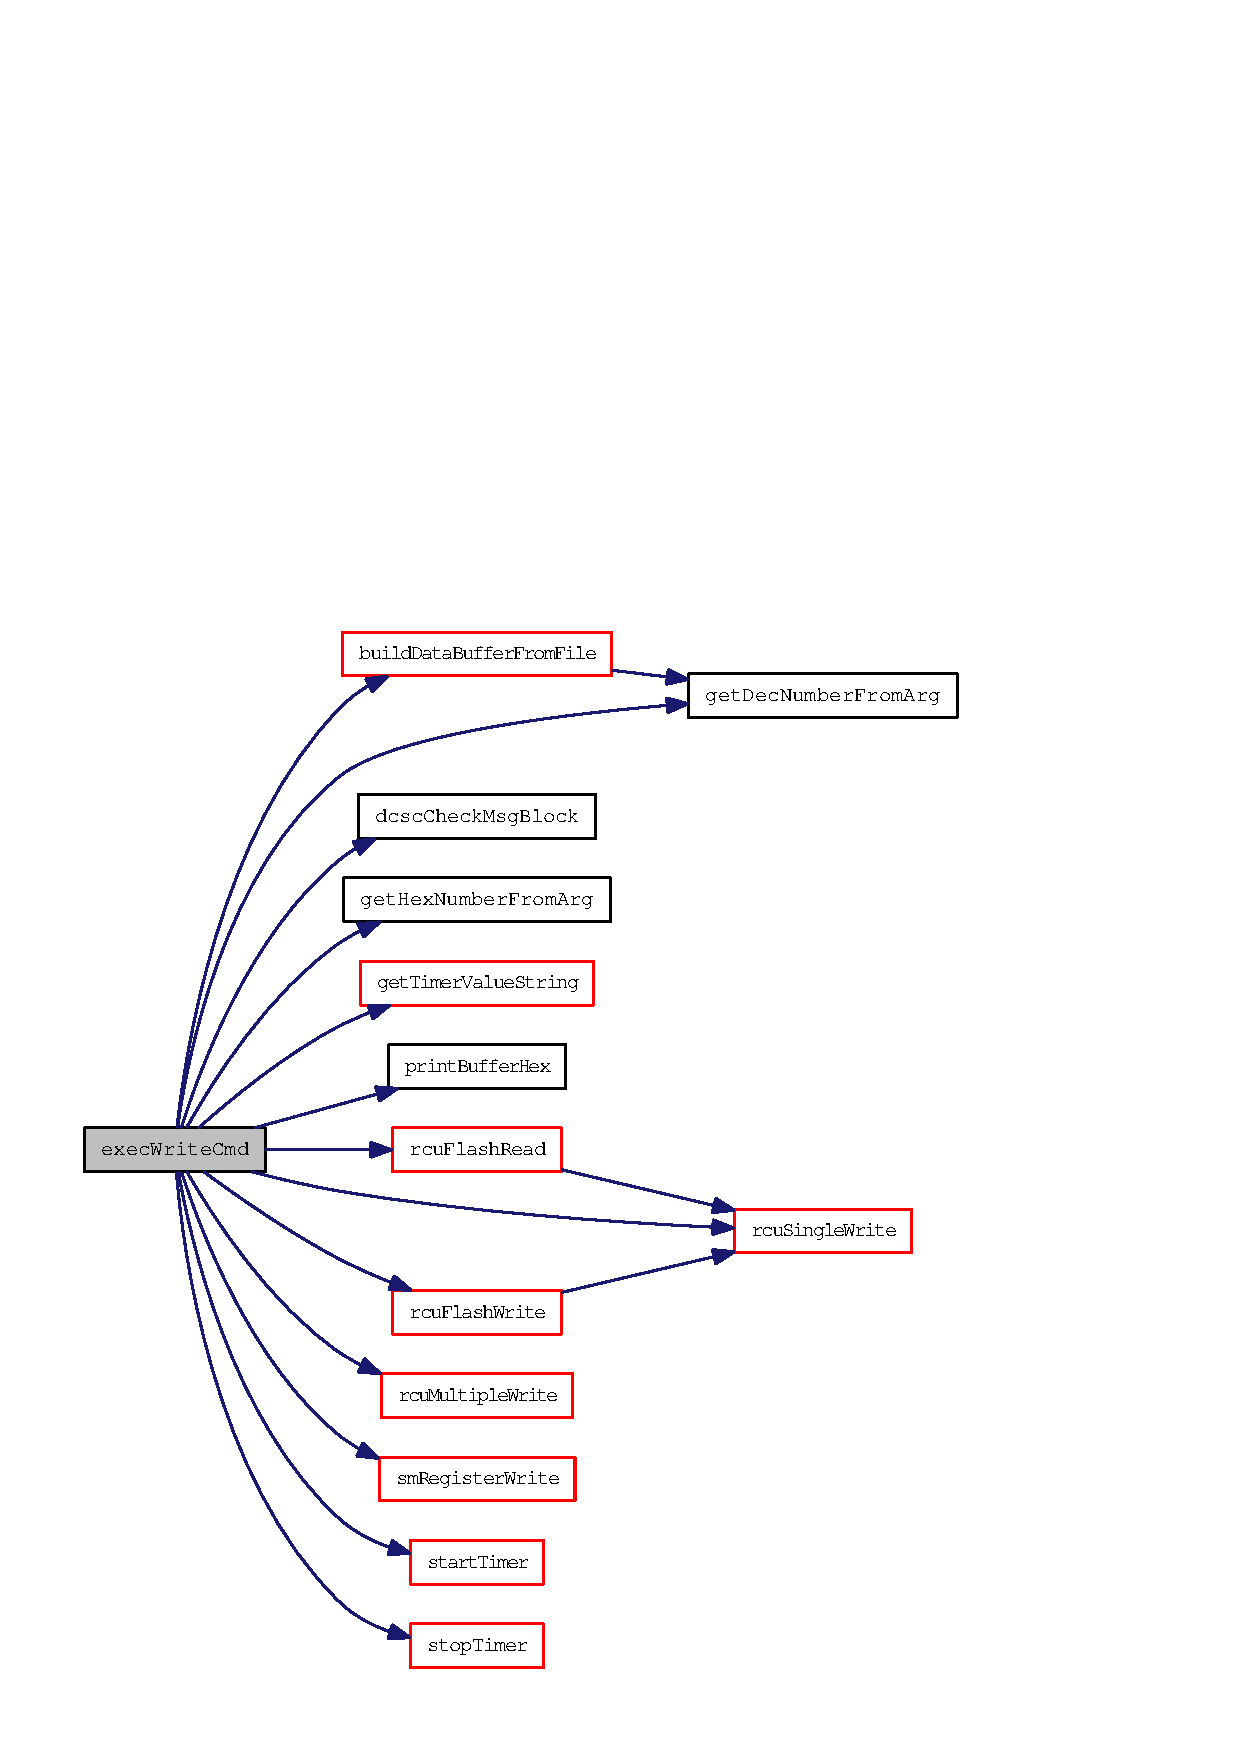
\includegraphics[width=232pt]{cmdInterpreter_8c_6f67c6327e24c23440e0fdf83d06e41d_cgraph}
\end{center}
\end{figure}
\hypertarget{cmdInterpreter_8c_c744cdcd05bdccf013ccbc82daa2282a}{
\index{cmdInterpreter.c@{cmd\-Interpreter.c}!printBatchProcHelp@{printBatchProcHelp}}
\index{printBatchProcHelp@{printBatchProcHelp}!cmdInterpreter.c@{cmd\-Interpreter.c}}
\subsubsection[printBatchProcHelp]{\setlength{\rightskip}{0pt plus 5cm}void print\-Batch\-Proc\-Help ()}}
\label{cmdInterpreter_8c_c744cdcd05bdccf013ccbc82daa2282a}




Definition at line 262 of file cmd\-Interpreter.c.

Referenced by execute\-Main\-Commands().\hypertarget{cmdInterpreter_8c_15843554cb32ffb674f4245cfe5ee524}{
\index{cmdInterpreter.c@{cmd\-Interpreter.c}!printDebugHelp@{printDebugHelp}}
\index{printDebugHelp@{printDebugHelp}!cmdInterpreter.c@{cmd\-Interpreter.c}}
\subsubsection[printDebugHelp]{\setlength{\rightskip}{0pt plus 5cm}void print\-Debug\-Help (int {\em i\-Level})}}
\label{cmdInterpreter_8c_15843554cb32ffb674f4245cfe5ee524}




Definition at line 173 of file cmd\-Interpreter.c.

References CHECK\_\-COMMAND\_\-BUFFER, DBG\_\-ARGUMENT\_\-CONVERT, DBG\_\-CHECK\_\-COMMAND, DBG\_\-DEFAULT, DBG\_\-FILE\_\-CONVERT, IGNORE\_\-BUFFER\_\-CHECK, PRINT\_\-COMMAND\_\-BUFFER, PRINT\_\-COMMAND\_\-RESULT, PRINT\_\-REGISTER\_\-ACCESS, PRINT\_\-RESULT\_\-BUFFER, PRINT\_\-RESULT\_\-HUMAN\_\-READABLE, and PRINT\_\-SPLIT\_\-DEBUG.

Referenced by execute\-Main\-Commands().\hypertarget{cmdInterpreter_8c_69279ab735c2dc7e0a73d9c0bfe44f20}{
\index{cmdInterpreter.c@{cmd\-Interpreter.c}!printFirmwareHelp@{printFirmwareHelp}}
\index{printFirmwareHelp@{printFirmwareHelp}!cmdInterpreter.c@{cmd\-Interpreter.c}}
\subsubsection[printFirmwareHelp]{\setlength{\rightskip}{0pt plus 5cm}int print\-Firmware\-Help ()}}
\label{cmdInterpreter_8c_69279ab735c2dc7e0a73d9c0bfe44f20}




Definition at line 1773 of file cmd\-Interpreter.c.\hypertarget{cmdInterpreter_8c_587fc3f8784e8339c998d9ca71bd7e12}{
\index{cmdInterpreter.c@{cmd\-Interpreter.c}!printFlashHelp@{printFlashHelp}}
\index{printFlashHelp@{printFlashHelp}!cmdInterpreter.c@{cmd\-Interpreter.c}}
\subsubsection[printFlashHelp]{\setlength{\rightskip}{0pt plus 5cm}int print\-Flash\-Help ()}}
\label{cmdInterpreter_8c_587fc3f8784e8339c998d9ca71bd7e12}




Definition at line 1677 of file cmd\-Interpreter.c.\hypertarget{cmdInterpreter_8c_f03f7609a66def2e7fae02a477c38d97}{
\index{cmdInterpreter.c@{cmd\-Interpreter.c}!printHelp@{printHelp}}
\index{printHelp@{printHelp}!cmdInterpreter.c@{cmd\-Interpreter.c}}
\subsubsection[printHelp]{\setlength{\rightskip}{0pt plus 5cm}int print\-Help ()}}
\label{cmdInterpreter_8c_f03f7609a66def2e7fae02a477c38d97}




Definition at line 198 of file cmd\-Interpreter.c.

Referenced by execute\-Main\-Commands().\hypertarget{cmdInterpreter_8c_ac3ae2fb745e63e33060d5c0b658f745}{
\index{cmdInterpreter.c@{cmd\-Interpreter.c}!printInfo@{printInfo}}
\index{printInfo@{printInfo}!cmdInterpreter.c@{cmd\-Interpreter.c}}
\subsubsection[printInfo]{\setlength{\rightskip}{0pt plus 5cm}int print\-Info ()}}
\label{cmdInterpreter_8c_ac3ae2fb745e63e33060d5c0b658f745}




Definition at line 164 of file cmd\-Interpreter.c.\hypertarget{cmdInterpreter_8c_17ba9ebf0687897855a7c95f19e99c3d}{
\index{cmdInterpreter.c@{cmd\-Interpreter.c}!printReadHelp@{printReadHelp}}
\index{printReadHelp@{printReadHelp}!cmdInterpreter.c@{cmd\-Interpreter.c}}
\subsubsection[printReadHelp]{\setlength{\rightskip}{0pt plus 5cm}void print\-Read\-Help ()}}
\label{cmdInterpreter_8c_17ba9ebf0687897855a7c95f19e99c3d}




Definition at line 240 of file cmd\-Interpreter.c.

Referenced by execute\-Main\-Commands().\hypertarget{cmdInterpreter_8c_e3bcc6695f3c41940a8ab1f428101f07}{
\index{cmdInterpreter.c@{cmd\-Interpreter.c}!printReadOutputFormatted@{printReadOutputFormatted}}
\index{printReadOutputFormatted@{printReadOutputFormatted}!cmdInterpreter.c@{cmd\-Interpreter.c}}
\subsubsection[printReadOutputFormatted]{\setlength{\rightskip}{0pt plus 5cm}int print\-Read\-Output\-Formatted (unsigned char $\ast$ {\em p\-Buffer}, int {\em i\-Buffer\-Size}, const char $\ast$ {\em p\-Format}, int {\em i\-Start\-Address}, FILE $\ast$ {\em fp})}}
\label{cmdInterpreter_8c_e3bcc6695f3c41940a8ab1f428101f07}




Definition at line 946 of file cmd\-Interpreter.c.

References DBG\_\-ARGUMENT\_\-CONVERT, INT\_\-RO\_\-MAX, Scan\-Coefficients(), set\-Debug\-Option\-Flag(), and UINT\_\-MAX.

Referenced by exec\-Read\-Cmd().

Here is the call graph for this function:\begin{figure}[H]
\begin{center}
\leavevmode
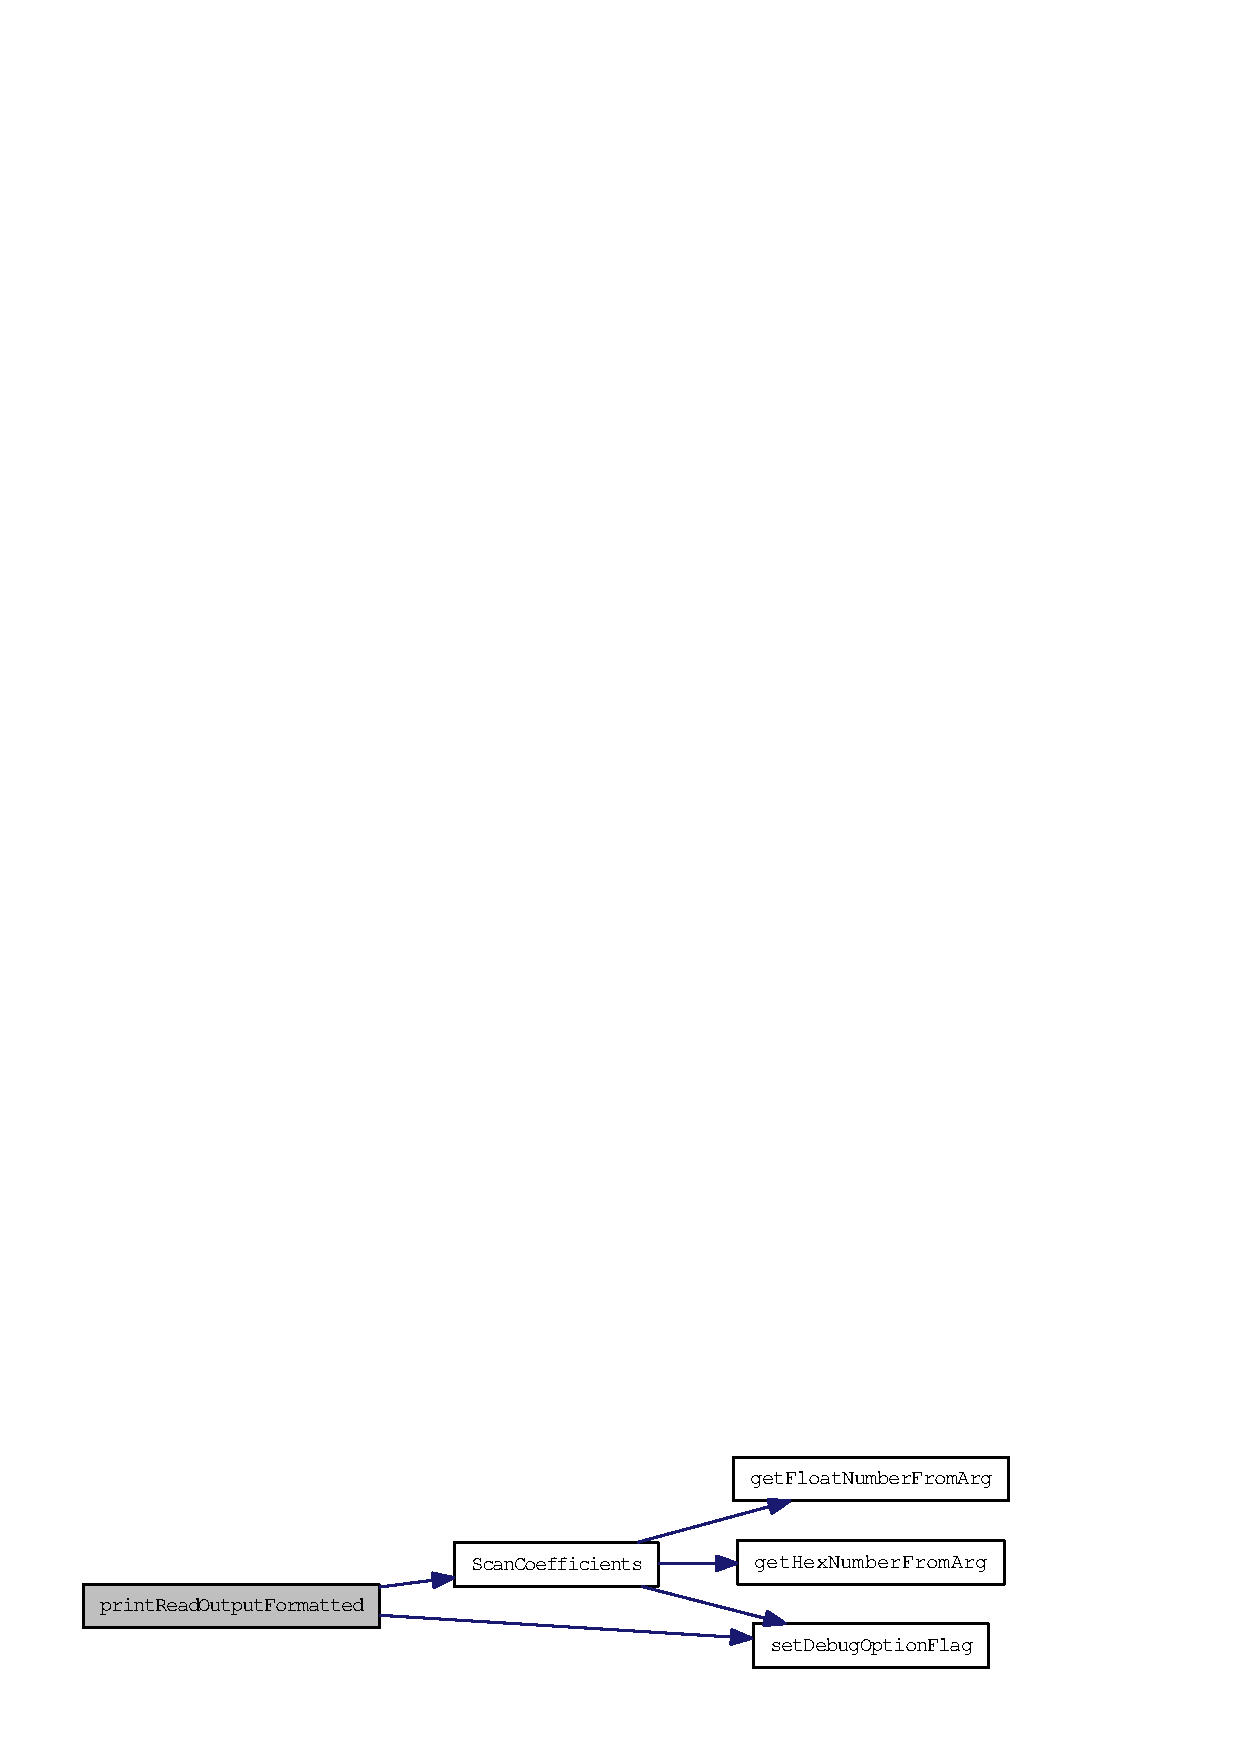
\includegraphics[width=244pt]{cmdInterpreter_8c_e3bcc6695f3c41940a8ab1f428101f07_cgraph}
\end{center}
\end{figure}
\hypertarget{cmdInterpreter_8c_76b0a4b334ee64eb25b1637d709deb92}{
\index{cmdInterpreter.c@{cmd\-Interpreter.c}!printSelectmapHelp@{printSelectmapHelp}}
\index{printSelectmapHelp@{printSelectmapHelp}!cmdInterpreter.c@{cmd\-Interpreter.c}}
\subsubsection[printSelectmapHelp]{\setlength{\rightskip}{0pt plus 5cm}int print\-Selectmap\-Help ()}}
\label{cmdInterpreter_8c_76b0a4b334ee64eb25b1637d709deb92}




Definition at line 1760 of file cmd\-Interpreter.c.\hypertarget{cmdInterpreter_8c_6ead18c93a106e1f1ba5871e908d9916}{
\index{cmdInterpreter.c@{cmd\-Interpreter.c}!readTime@{readTime}}
\index{readTime@{readTime}!cmdInterpreter.c@{cmd\-Interpreter.c}}
\subsubsection[readTime]{\setlength{\rightskip}{0pt plus 5cm}int read\-Time (const char $\ast$$\ast$ {\em array\-Arg}, int {\em i\-Nof\-Args}, int $\ast$ {\em p\-Sec}, int $\ast$ {\em p\-Musec})}}
\label{cmdInterpreter_8c_6ead18c93a106e1f1ba5871e908d9916}




Definition at line 273 of file cmd\-Interpreter.c.

Referenced by exec\-Batch(), execute\-Main\-Commands(), and wait\-Condition().\hypertarget{cmdInterpreter_8c_78a2282cf7d3dbf552e5f9876dba01cf}{
\index{cmdInterpreter.c@{cmd\-Interpreter.c}!ScanCoefficients@{ScanCoefficients}}
\index{ScanCoefficients@{ScanCoefficients}!cmdInterpreter.c@{cmd\-Interpreter.c}}
\subsubsection[ScanCoefficients]{\setlength{\rightskip}{0pt plus 5cm}int Scan\-Coefficients (const char $\ast$ {\em p\-Format}, float $\ast$ {\em pf\-M}, float $\ast$ {\em pf\-N}, \_\-\_\-u32 $\ast$ {\em p\-Mask})}}
\label{cmdInterpreter_8c_78a2282cf7d3dbf552e5f9876dba01cf}




Definition at line 862 of file cmd\-Interpreter.c.

References DBG\_\-ARGUMENT\_\-CONVERT, get\-Float\-Number\-From\-Arg(), get\-Hex\-Number\-From\-Arg(), and set\-Debug\-Option\-Flag().

Referenced by print\-Read\-Output\-Formatted().

Here is the call graph for this function:\begin{figure}[H]
\begin{center}
\leavevmode
\includegraphics[width=155pt]{cmdInterpreter_8c_78a2282cf7d3dbf552e5f9876dba01cf_cgraph}
\end{center}
\end{figure}
\hypertarget{cmdInterpreter_8c_ae37490e691f5b4d2c2e8f22713555da}{
\index{cmdInterpreter.c@{cmd\-Interpreter.c}!terminateBatchProcessing@{terminateBatchProcessing}}
\index{terminateBatchProcessing@{terminateBatchProcessing}!cmdInterpreter.c@{cmd\-Interpreter.c}}
\subsubsection[terminateBatchProcessing]{\setlength{\rightskip}{0pt plus 5cm}int terminate\-Batch\-Processing ()}}
\label{cmdInterpreter_8c_ae37490e691f5b4d2c2e8f22713555da}




Definition at line 1280 of file cmd\-Interpreter.c.

References g\_\-b\-Batch\-Processing.

Referenced by sigquit\-Handler().\hypertarget{cmdInterpreter_8c_ac7fb947e83d5813fb30995133f29955}{
\index{cmdInterpreter.c@{cmd\-Interpreter.c}!timedWait@{timedWait}}
\index{timedWait@{timedWait}!cmdInterpreter.c@{cmd\-Interpreter.c}}
\subsubsection[timedWait]{\setlength{\rightskip}{0pt plus 5cm}int timed\-Wait (int {\em i\-Wait\-Sec}, int {\em i\-Wait\-Musec})}}
\label{cmdInterpreter_8c_ac7fb947e83d5813fb30995133f29955}




Definition at line 1252 of file cmd\-Interpreter.c.

References get\-Timer\-Value(), start\-Timer(), and stop\-Timer().

Referenced by exec\-Batch(), and execute\-Main\-Commands().

Here is the call graph for this function:\begin{figure}[H]
\begin{center}
\leavevmode
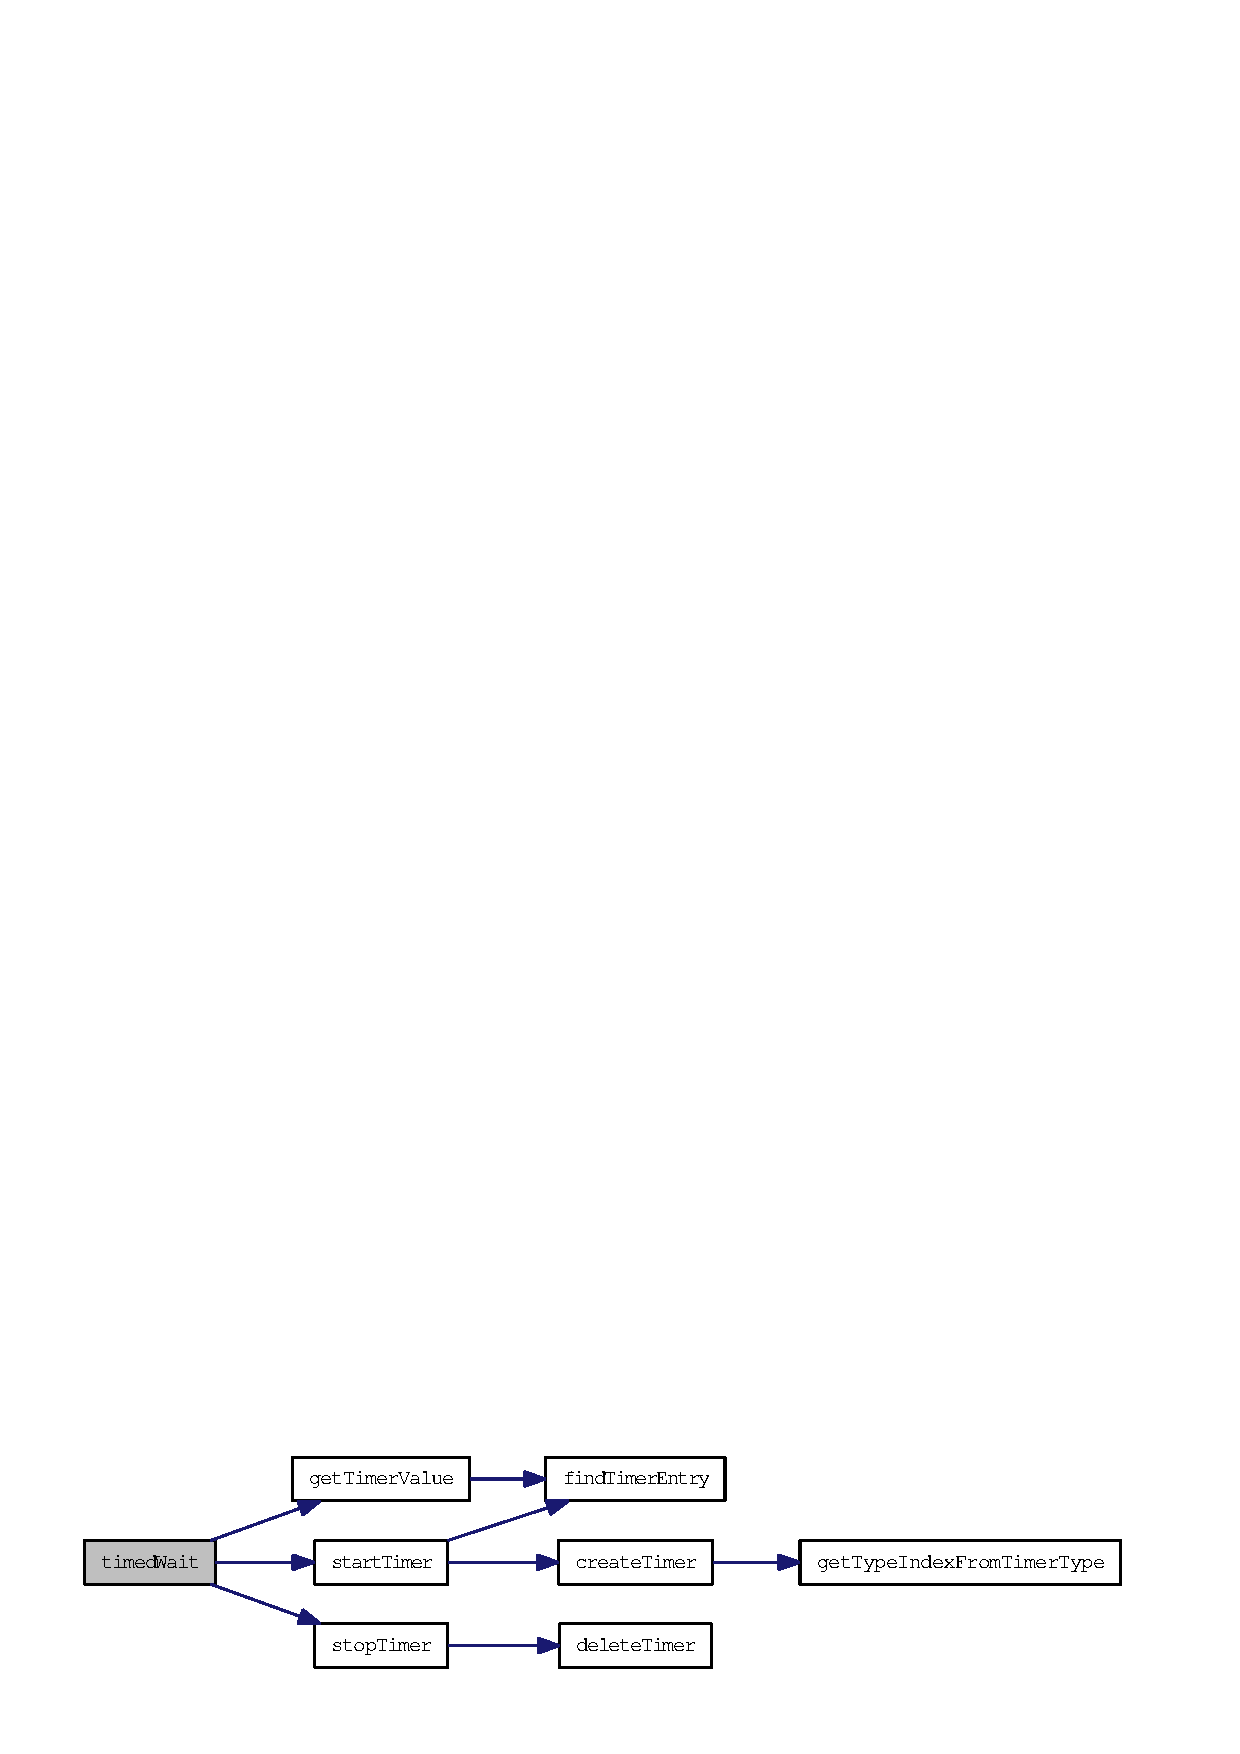
\includegraphics[width=271pt]{cmdInterpreter_8c_ac7fb947e83d5813fb30995133f29955_cgraph}
\end{center}
\end{figure}
\hypertarget{cmdInterpreter_8c_a78c9a935a342b0b7b9a3c9896c5e85b}{
\index{cmdInterpreter.c@{cmd\-Interpreter.c}!waitCondition@{waitCondition}}
\index{waitCondition@{waitCondition}!cmdInterpreter.c@{cmd\-Interpreter.c}}
\subsubsection[waitCondition]{\setlength{\rightskip}{0pt plus 5cm}int wait\-Condition (const char $\ast$$\ast$ {\em array\-Arg}, int {\em i\-Nof\-Args})}}
\label{cmdInterpreter_8c_a78c9a935a342b0b7b9a3c9896c5e85b}




Definition at line 304 of file cmd\-Interpreter.c.

References DBG\_\-ARGUMENT\_\-CONVERT, DBG\_\-CHECK\_\-COMMAND, e\_\-continue, e\_\-fail, get\-Hex\-Number\-From\-Arg(), get\-Timer\-Value(), rcu\-Single\-Read(), read\-Time(), set\-Debug\-Option\-Flag(), start\-Simulation(), start\-Timer(), stop\-Simulation(), stop\-Timer(), and TCondition::type.

Referenced by execute\-Main\-Commands().

Here is the call graph for this function:\begin{figure}[H]
\begin{center}
\leavevmode
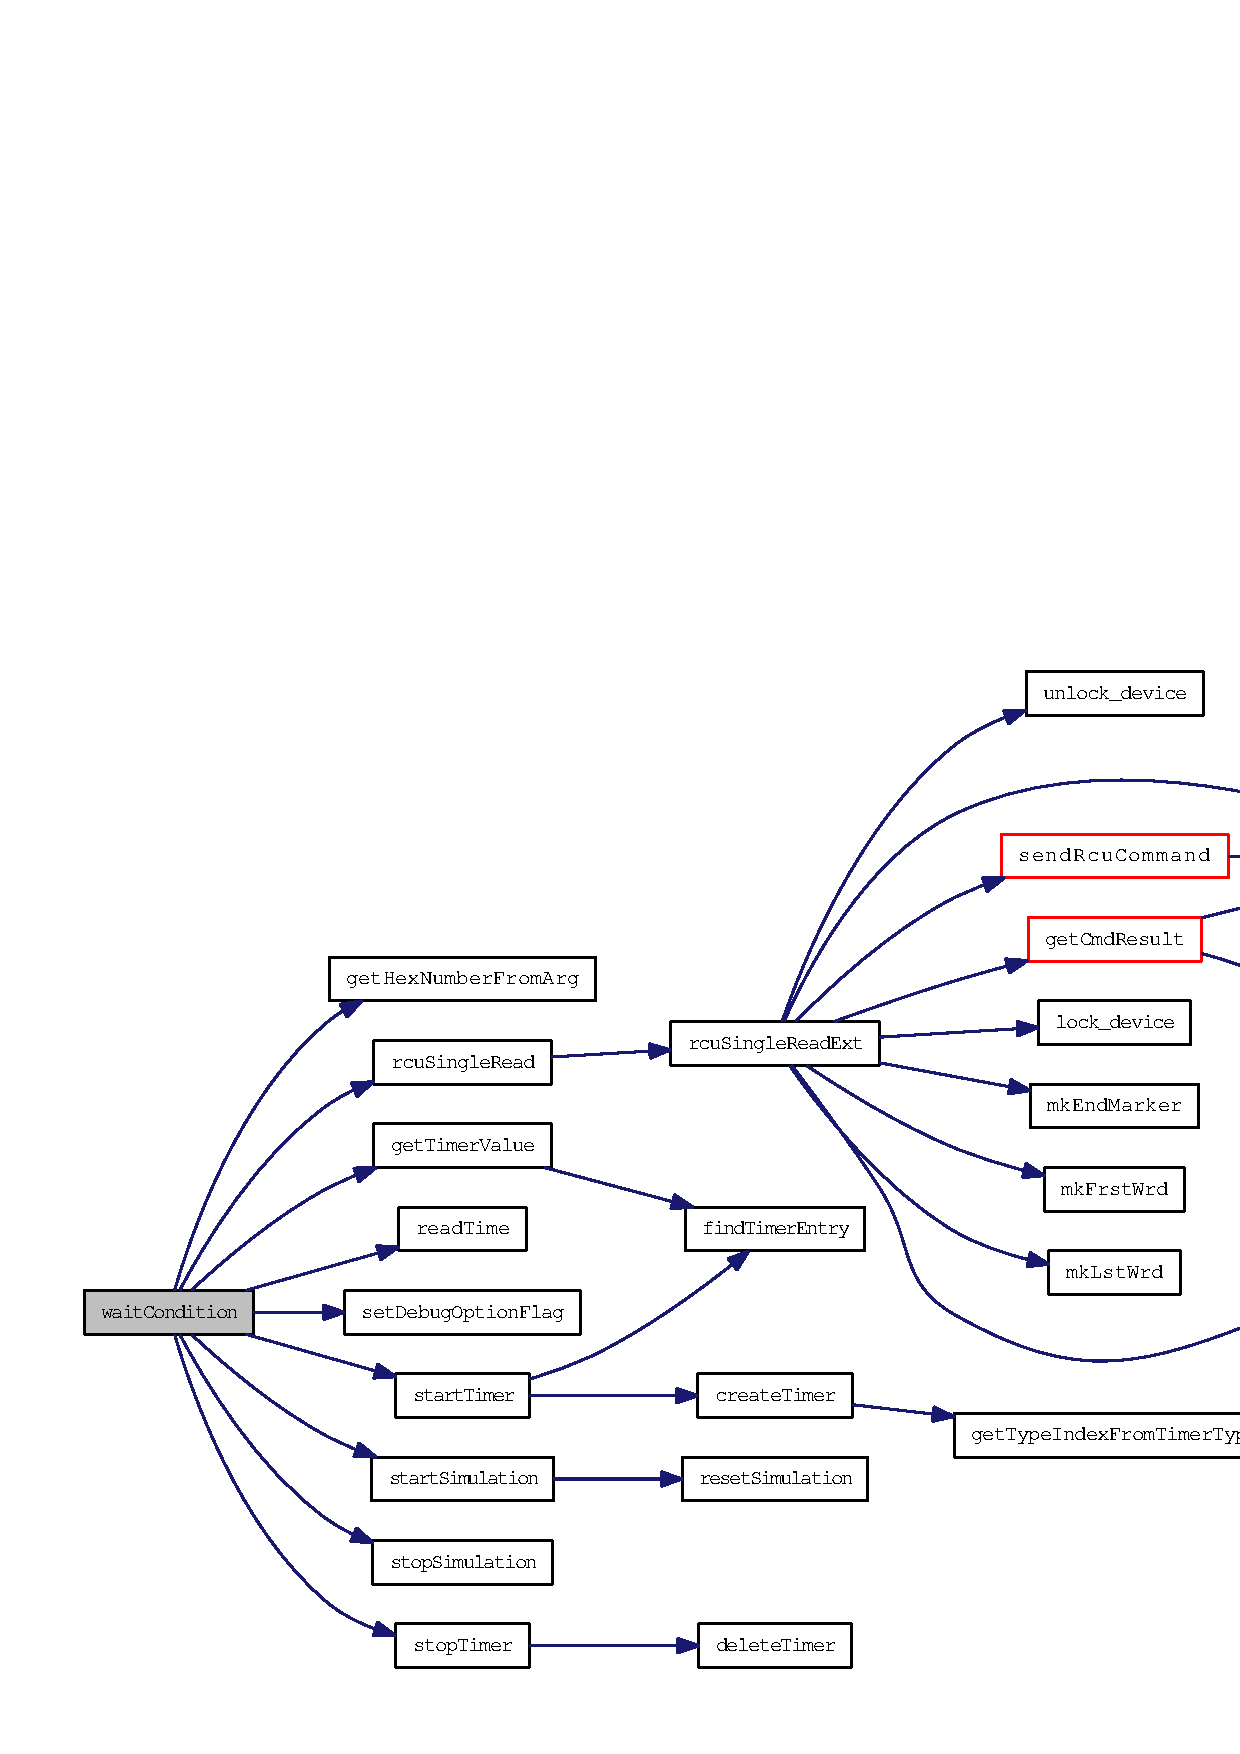
\includegraphics[width=374pt]{cmdInterpreter_8c_a78c9a935a342b0b7b9a3c9896c5e85b_cgraph}
\end{center}
\end{figure}


\subsection{Variable Documentation}
\hypertarget{cmdInterpreter_8c_c1784239c15c2f1b5b4f1dbda9df65e7}{
\index{cmdInterpreter.c@{cmd\-Interpreter.c}!ctrlRegCmds@{ctrlRegCmds}}
\index{ctrlRegCmds@{ctrlRegCmds}!cmdInterpreter.c@{cmd\-Interpreter.c}}
\subsubsection[ctrlRegCmds]{\setlength{\rightskip}{0pt plus 5cm}\hyperlink{structArgDef__t}{TArg\-Def} \hyperlink{cmdInterpreter_8c_c1784239c15c2f1b5b4f1dbda9df65e7}{ctrl\-Reg\-Cmds}\mbox{[}$\,$\mbox{]}}}
\label{cmdInterpreter_8c_c1784239c15c2f1b5b4f1dbda9df65e7}


\textbf{Initial value:}

\begin{Code}\begin{verbatim} {
  {"","",{eUnknownType, {NULL}},{NULL},ARGDEF_TERMINATE},
}
\end{verbatim}\end{Code}


Definition at line 1876 of file cmd\-Interpreter.c.\hypertarget{cmdInterpreter_8c_083a182722ef62f10a68012ab6d7f707}{
\index{cmdInterpreter.c@{cmd\-Interpreter.c}!driverCtrlArgs@{driverCtrlArgs}}
\index{driverCtrlArgs@{driverCtrlArgs}!cmdInterpreter.c@{cmd\-Interpreter.c}}
\subsubsection[driverCtrlArgs]{\setlength{\rightskip}{0pt plus 5cm}\hyperlink{structArgDef__t}{TArg\-Def} \hyperlink{cmdInterpreter_8c_083a182722ef62f10a68012ab6d7f707}{driver\-Ctrl\-Args}\mbox{[}$\,$\mbox{]}}}
\label{cmdInterpreter_8c_083a182722ef62f10a68012ab6d7f707}


\textbf{Initial value:}

\begin{Code}\begin{verbatim} {
  {"i","info",{eFctIndex, {(void*)printDriverInfo}},{(void*)1},ARGDEF_BREAK},
  {"l","lock",{eFctIndex, {(void*)dcscLockCtrl}},{(void*)eLock},ARGDEF_BREAK},
  {"u","unlock",{eFctIndex, {(void*)dcscLockCtrl}},{(void*)eUnlock},ARGDEF_BREAK},
  {"r","reset",{eFctIndex, {(void*)dcscLockCtrl}},{(void*)eDeactivateLock},ARGDEF_BREAK},
  {"a","activate",{eFctIndex, {(void*)dcscLockCtrl}},{(void*)eActivateLock},ARGDEF_BREAK},
  {NULL,"seize",{eFctIndex, {(void*)dcscLockCtrl}},{(void*)eSeize},ARGDEF_BREAK},
  {NULL,"release",{eFctIndex, {(void*)dcscLockCtrl}},{(void*)eRelease},ARGDEF_BREAK},
  {NULL,"debug",{eHex, {NULL}},{NULL},ARGDEF_BREAK},
  {"","",{eUnknownType, {NULL}},{NULL},ARGDEF_TERMINATE},
}
\end{verbatim}\end{Code}


Definition at line 1427 of file cmd\-Interpreter.c.\hypertarget{cmdInterpreter_8c_3e75245c450c10d2323442d359f053d7}{
\index{cmdInterpreter.c@{cmd\-Interpreter.c}!driverCtrlDesc@{driverCtrlDesc}}
\index{driverCtrlDesc@{driverCtrlDesc}!cmdInterpreter.c@{cmd\-Interpreter.c}}
\subsubsection[driverCtrlDesc]{\setlength{\rightskip}{0pt plus 5cm}\hyperlink{structFctArg__t}{TFct\-Arg} \hyperlink{cmdInterpreter_8c_3e75245c450c10d2323442d359f053d7}{driver\-Ctrl\-Desc}}}
\label{cmdInterpreter_8c_3e75245c450c10d2323442d359f053d7}


\textbf{Initial value:}

\begin{Code}\begin{verbatim} {
  driverCtrlArgs,
  NULL,
  NULL
}
\end{verbatim}\end{Code}


Definition at line 1439 of file cmd\-Interpreter.c.\hypertarget{cmdInterpreter_8c_5a94aee581a390576806909f67968c30}{
\index{cmdInterpreter.c@{cmd\-Interpreter.c}!firmwareCmds@{firmwareCmds}}
\index{firmwareCmds@{firmwareCmds}!cmdInterpreter.c@{cmd\-Interpreter.c}}
\subsubsection[firmwareCmds]{\setlength{\rightskip}{0pt plus 5cm}\hyperlink{structArgDef__t}{TArg\-Def} \hyperlink{cmdInterpreter_8c_5a94aee581a390576806909f67968c30}{firmware\-Cmds}\mbox{[}$\,$\mbox{]}}}
\label{cmdInterpreter_8c_5a94aee581a390576806909f67968c30}


\textbf{Initial value:}

\begin{Code}\begin{verbatim} {
  {"r","reset",{eFctIndex, {(void*)rcuBusControlCmd}},{(void*)eResetFirmware},ARGDEF_TERMINATE},
  {"wr","write-reg",{eFctUserScan, {(void*)execRegWriteCmd}},{NULL},ARGDEF_TERMINATE},
  {"rr","read-reg", {eFctUserScan, {(void*)execRegReadCmd}}, {NULL},ARGDEF_TERMINATE},
  {"ec","enable-comp",{eFctIndex, {(void*)rcuBusControlCmd}},{(void*)eEnableCompression},ARGDEF_TERMINATE},
  {"dc","enable-comp",{eFctIndex, {(void*)rcuBusControlCmd}},{(void*)eDisableCompression},ARGDEF_TERMINATE},
  {"*",NULL,{eFctNoArg, {(void*)printFirmwareHelp}},{NULL},ARGDEF_TERMINATE},
  {"","",{eUnknownType, {NULL}},{NULL},ARGDEF_TERMINATE},
}
\end{verbatim}\end{Code}


Definition at line 1866 of file cmd\-Interpreter.c.\hypertarget{cmdInterpreter_8c_5a3ddbaacf0c338e408e3c0b55189d58}{
\index{cmdInterpreter.c@{cmd\-Interpreter.c}!flashCmds@{flashCmds}}
\index{flashCmds@{flashCmds}!cmdInterpreter.c@{cmd\-Interpreter.c}}
\subsubsection[flashCmds]{\setlength{\rightskip}{0pt plus 5cm}\hyperlink{structArgDef__t}{TArg\-Def} \hyperlink{cmdInterpreter_8c_5a3ddbaacf0c338e408e3c0b55189d58}{flash\-Cmds}\mbox{[}$\,$\mbox{]}}}
\label{cmdInterpreter_8c_5a3ddbaacf0c338e408e3c0b55189d58}


\textbf{Initial value:}

\begin{Code}\begin{verbatim} {
  {"e","enable",{eFctIndex, {(void*)rcuBusControlCmd}},{(void*)eEnableFlash},ARGDEF_TERMINATE},
  {"d","disable",{eFctIndex, {(void*)rcuBusControlCmd}},{(void*)eDisableFlash},ARGDEF_TERMINATE},
  {NULL,"reset",{eFctIndex, {(void*)rcuBusControlCmd}},{(void*)eResetFlash},ARGDEF_TERMINATE},
  {NULL,"id",{eFctIndex, {(void*)rcuBusControlCmd}},{(void*)eFlashID},ARGDEF_TERMINATE},
  {NULL,"ctrldcs",{eFctIndex, {(void*)rcuBusControlCmd}},{(void*)eFlashCtrlDCS},ARGDEF_TERMINATE},
  {NULL,"ctrlactel",{eFctIndex, {(void*)rcuBusControlCmd}},{(void*)eFlashCtrlActel},ARGDEF_TERMINATE},
  {"w","write",{eFctUserScan, {(void*)execFlashWriteCmd}},{NULL},ARGDEF_TERMINATE},
  {"r","read",{eFctUserScan, {(void*)execFlashReadCmd}},{NULL},ARGDEF_TERMINATE},
  {"v","verify",{eFctUserScan, {(void*)execFlashVerifyCmd}},{NULL},ARGDEF_TERMINATE},
  {NULL,"erase",{eFctArgDef, {(void*)execFlashErase}},{(void*)&flashEraseDesc},ARGDEF_TERMINATE},
  {NULL,"eraseall",{eFctNoArg, {(void*)execFlashEraseall}},{NULL},ARGDEF_TERMINATE},
  {"*",NULL,{eFctNoArg, {(void*)printFlashHelp}},{NULL},ARGDEF_TERMINATE},
  {"","",{eUnknownType, {NULL}},{NULL},ARGDEF_TERMINATE},
}
\end{verbatim}\end{Code}


Definition at line 1850 of file cmd\-Interpreter.c.\hypertarget{cmdInterpreter_8c_9a757fd68a4d59000e0938fcdb423996}{
\index{cmdInterpreter.c@{cmd\-Interpreter.c}!flashEraseDesc@{flashEraseDesc}}
\index{flashEraseDesc@{flashEraseDesc}!cmdInterpreter.c@{cmd\-Interpreter.c}}
\subsubsection[flashEraseDesc]{\setlength{\rightskip}{0pt plus 5cm}\hyperlink{structFctArg__t}{TFct\-Arg} \hyperlink{cmdInterpreter_8c_9a757fd68a4d59000e0938fcdb423996}{flash\-Erase\-Desc}}}
\label{cmdInterpreter_8c_9a757fd68a4d59000e0938fcdb423996}


\textbf{Initial value:}

\begin{Code}\begin{verbatim} {
  flashEraseParams,
  NULL,
  NULL
}
\end{verbatim}\end{Code}


Definition at line 1844 of file cmd\-Interpreter.c.\hypertarget{cmdInterpreter_8c_7399e2dab99f698c9275622762e94f74}{
\index{cmdInterpreter.c@{cmd\-Interpreter.c}!flashEraseParams@{flashEraseParams}}
\index{flashEraseParams@{flashEraseParams}!cmdInterpreter.c@{cmd\-Interpreter.c}}
\subsubsection[flashEraseParams]{\setlength{\rightskip}{0pt plus 5cm}\hyperlink{structArgDef__t}{TArg\-Def} \hyperlink{cmdInterpreter_8c_7399e2dab99f698c9275622762e94f74}{flash\-Erase\-Params}\mbox{[}$\,$\mbox{]}}}
\label{cmdInterpreter_8c_7399e2dab99f698c9275622762e94f74}


\textbf{Initial value:}

\begin{Code}\begin{verbatim} {
  {NULL,"all",{eBool, {(void*)0}},{(void*)NULL},ARGDEF_BREAK},
  {"sec","sector",{eHex, {(void*)0}},{(void*)NULL},0},
  {NULL,"_count",{eInteger, {(void*)0}},{(void*)NULL},ARGDEF_RESUME|ARGDEF_KEYWORDLESS},
  {"","",{eUnknownType, {NULL}},{NULL},ARGDEF_TERMINATE},
}
\end{verbatim}\end{Code}


Definition at line 1837 of file cmd\-Interpreter.c.\hypertarget{cmdInterpreter_8c_0aee2ec97f7e88992f9b2b333ca99be2}{
\index{cmdInterpreter.c@{cmd\-Interpreter.c}!g_bBatchProcessing@{g\_\-bBatchProcessing}}
\index{g_bBatchProcessing@{g\_\-bBatchProcessing}!cmdInterpreter.c@{cmd\-Interpreter.c}}
\subsubsection[g\_\-bBatchProcessing]{\setlength{\rightskip}{0pt plus 5cm}int \hyperlink{cmdInterpreter_8c_0aee2ec97f7e88992f9b2b333ca99be2}{g\_\-b\-Batch\-Processing} = 0}}
\label{cmdInterpreter_8c_0aee2ec97f7e88992f9b2b333ca99be2}




Definition at line 1279 of file cmd\-Interpreter.c.

Referenced by exec\-Batch(), and terminate\-Batch\-Processing().\hypertarget{cmdInterpreter_8c_b1b44b602185677d4a2a372121627437}{
\index{cmdInterpreter.c@{cmd\-Interpreter.c}!g_profiling@{g\_\-profiling}}
\index{g_profiling@{g\_\-profiling}!cmdInterpreter.c@{cmd\-Interpreter.c}}
\subsubsection[g\_\-profiling]{\setlength{\rightskip}{0pt plus 5cm}int \hyperlink{cmdInterpreter_8c_b1b44b602185677d4a2a372121627437}{g\_\-profiling} = 0}}
\label{cmdInterpreter_8c_b1b44b602185677d4a2a372121627437}




Definition at line 60 of file cmd\-Interpreter.c.

Referenced by exec\-Batch(), execute\-Main\-Commands(), and exec\-Write\-Cmd().\hypertarget{cmdInterpreter_8c_014d78494c13d4dc0430ee68de158559}{
\index{cmdInterpreter.c@{cmd\-Interpreter.c}!mainCommands@{mainCommands}}
\index{mainCommands@{mainCommands}!cmdInterpreter.c@{cmd\-Interpreter.c}}
\subsubsection[mainCommands]{\setlength{\rightskip}{0pt plus 5cm}\hyperlink{structArgDef__t}{TArg\-Def} \hyperlink{cmdInterpreter_8c_014d78494c13d4dc0430ee68de158559}{main\-Commands}\mbox{[}$\,$\mbox{]}}}
\label{cmdInterpreter_8c_014d78494c13d4dc0430ee68de158559}


\textbf{Initial value:}

\begin{Code}\begin{verbatim} {
  {"sm","selectmap",{eFctRemaining, {(void*)selectmapCmds}},{(void*)&scanModeDefault},ARGDEF_TERMINATE},
  {NULL,"flash",{eFctRemaining, {(void*)flashCmds}},{(void*)&scanModeDefault},ARGDEF_TERMINATE},
  {"fw","firmware",{eFctRemaining, {(void*)firmwareCmds}},{(void*)&scanModeDefault},ARGDEF_TERMINATE},
  {"rcr","read-ctrlreg",{eFctNoArg, {(void*)ctrlRegStatus}},{NULL},ARGDEF_TERMINATE},
  {"d","driver",{eFctArgDef, {(void*)driverCtrlCmds}},{(void*)&driverCtrlDesc},ARGDEF_TERMINATE},
  {"i","info",{eFctNoArg, {(void*)printInfo}},{NULL},ARGDEF_TERMINATE},
  {"#",NULL,{eBool, {NULL}},{NULL},ARGDEF_TERMINATE},
  {NULL,"*",{eFctUserScan, {(void*)executeMainCommands}},{NULL},ARGDEF_TERMINATE},
  {"","",{eUnknownType, {NULL}},{NULL},ARGDEF_TERMINATE},
}
\end{verbatim}\end{Code}


Definition at line 1880 of file cmd\-Interpreter.c.

Referenced by execute\-Command\-Args().\hypertarget{cmdInterpreter_8c_fbc09bb85c6e4618a38dba855c588abd}{
\index{cmdInterpreter.c@{cmd\-Interpreter.c}!scanModeDefault@{scanModeDefault}}
\index{scanModeDefault@{scanModeDefault}!cmdInterpreter.c@{cmd\-Interpreter.c}}
\subsubsection[scanModeDefault]{\setlength{\rightskip}{0pt plus 5cm}\hyperlink{structFctMode__t}{TFct\-Mode} \hyperlink{cmdInterpreter_8c_fbc09bb85c6e4618a38dba855c588abd}{scan\-Mode\-Default} = \{SCANMODE\_\-FORCE\_\-TERMINATION, NULL, NULL\}}}
\label{cmdInterpreter_8c_fbc09bb85c6e4618a38dba855c588abd}




Definition at line 1826 of file cmd\-Interpreter.c.\hypertarget{cmdInterpreter_8c_4954a4ac4d6f82836d8b405a2ec86071}{
\index{cmdInterpreter.c@{cmd\-Interpreter.c}!selectmapCmds@{selectmapCmds}}
\index{selectmapCmds@{selectmapCmds}!cmdInterpreter.c@{cmd\-Interpreter.c}}
\subsubsection[selectmapCmds]{\setlength{\rightskip}{0pt plus 5cm}\hyperlink{structArgDef__t}{TArg\-Def} \hyperlink{cmdInterpreter_8c_4954a4ac4d6f82836d8b405a2ec86071}{selectmap\-Cmds}\mbox{[}$\,$\mbox{]}}}
\label{cmdInterpreter_8c_4954a4ac4d6f82836d8b405a2ec86071}


\textbf{Initial value:}

\begin{Code}\begin{verbatim} {
  {"e","enable",{eFctIndex, {(void*)rcuBusControlCmd}},{(void*)eEnableSelectmap},ARGDEF_TERMINATE},
  {"d","disable",{eFctIndex, {(void*)rcuBusControlCmd}},{(void*)eDisableSelectmap},ARGDEF_TERMINATE},
  {"wr","write-reg",{eFctUserScan, {(void*)execSmWriteReg}},{NULL},ARGDEF_TERMINATE},
  {"rr","read-reg",{eFctUserScan, {(void*)execSmReadReg}},{NULL},ARGDEF_TERMINATE},
  {"*",NULL,{eFctNoArg, {(void*)printSelectmapHelp}},{NULL},ARGDEF_TERMINATE},
  {"","",{eUnknownType, {NULL}},{NULL},ARGDEF_TERMINATE},
}
\end{verbatim}\end{Code}


Definition at line 1828 of file cmd\-Interpreter.c.